\section{Results and Discussion}
\label{sec:result_and_discussion}

%----------------------------------------------------%
% --------- Brief Descriptive Statistics ---------%
%----------------------------------------------------%

\subsection{Brief Descriptive Statistics}
The review identified 61 articles published between 2004 and 2024. Scientific output in this area has accelerated in recent years, with the majority of papers published after 2020. Illustrated in Figure \ref{fig:scientific_productivity}, the number of published papers matching the screening criteria has increased significantly in recent years, peaking in 2024 with 13 publications after a rapid growth since 2018. Thus, it is possible that the field has advanced significantly in the later years, underscoring the need for a comprehensive literature review.

\begin{figure}[H]
    \centering
    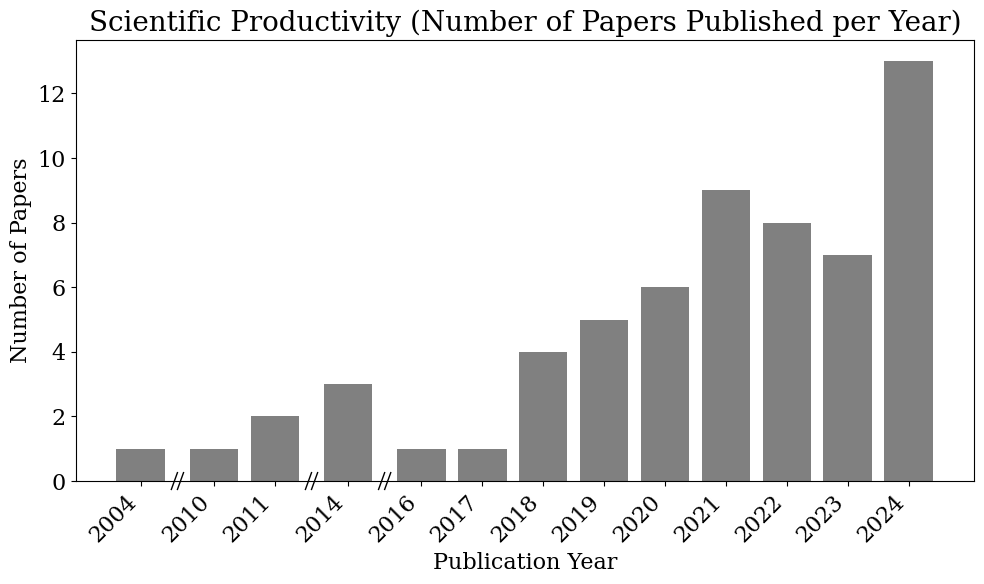
\includegraphics[width=1\linewidth]{Images/scientific_productivity.png}
    \caption{Annual distribution of papers in the field published included in the sample, illustrating the recent increase in publications}
    \label{fig:scientific_productivity}
\end{figure}

The majority of research originates from China, South-Korea and the US, with 16, 8 and 8 papers contributed by authors from these countries, respectively, as shown in Figure \ref{fig:author_country_origin_per_paper}. Each country is counted only once per paper, regardless of the number of contributing authors from that country.  

\begin{figure}[H]
    \centering
    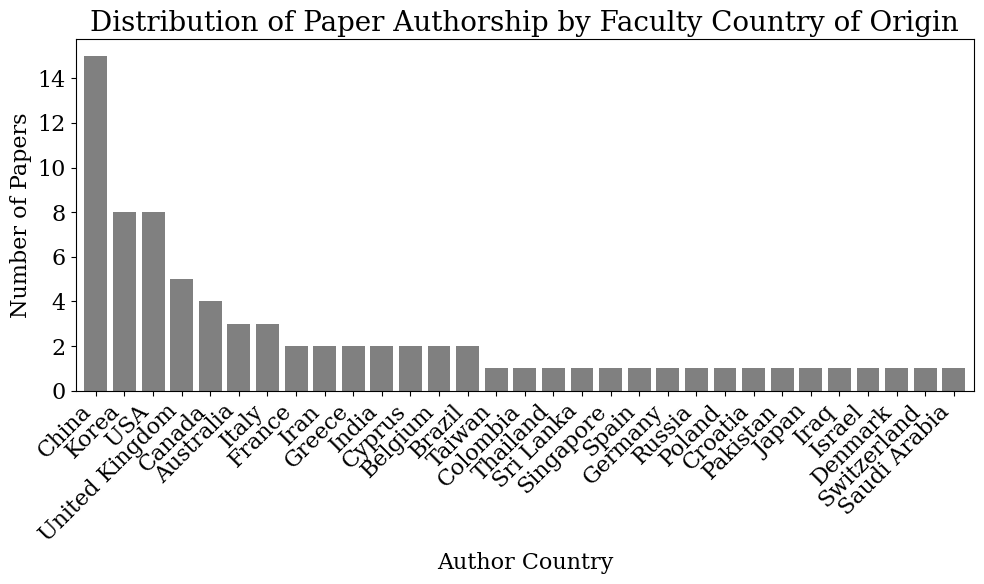
\includegraphics[width=1\linewidth]{Images/author_country_origin_per_paper.png}
    \caption{Number of articles by authors' faculty country of origin, with each country counted once per article to reflect international collaboration.}
    \label{fig:author_country_origin_per_paper}
\end{figure}

Notably, significant contributions to the field are made by authors from computer science and technical faculties, while only 20\% of authors have a background from financial, business or economics faculties, as illustrated in Figure \ref{fig:author_faculty_origin}. To capture the full scope of expertise, all authors are counted individually. 


\begin{figure}[H]
    \centering
    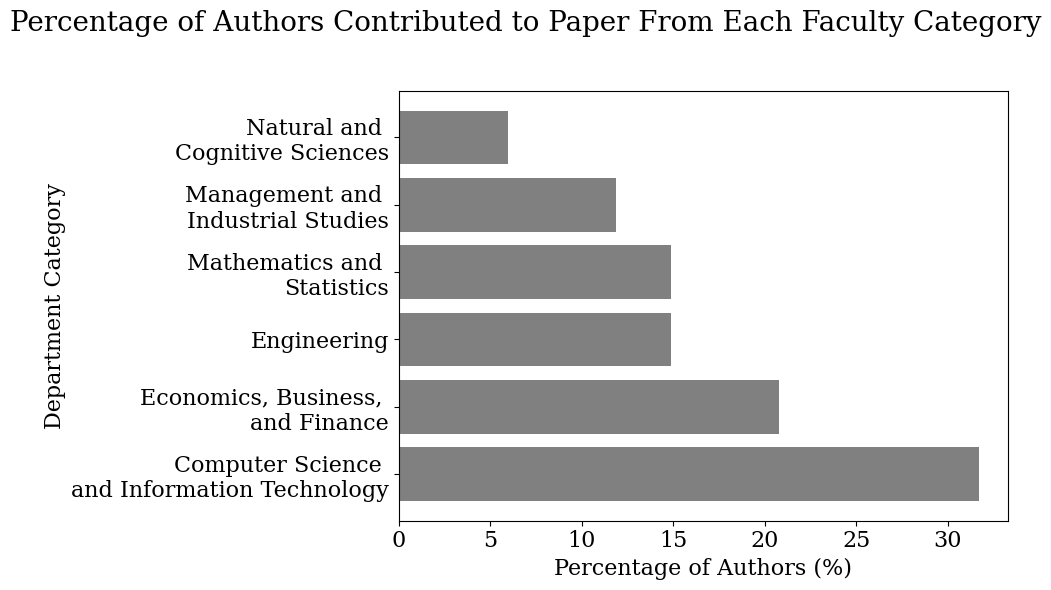
\includegraphics[width=1\linewidth]{Images/author_faculty_origin.png}
    \caption{Percentage distribution of authors by faculty category.}
    \label{fig:author_faculty_origin}
\end{figure}

In terms of journal origins, the majority of the papers from the sample were published in engineering, technical, computer science, and artificial intelligence journals or others. There are only a minor representation in finance and economics journals (14 out of 61 papers). Figure \ref{fig:num_papers_per_journal_category} shows the distribution of publications across journal categories. This distribution could suggest a potential gap in domain-specific financial research, indicating an opportunity for increased financial focused journal contributions. The categorizing of journals is detailed in Appendix \ref{appendix:journal_category_mapping}. 

\begin{figure}[H]
    \centering
    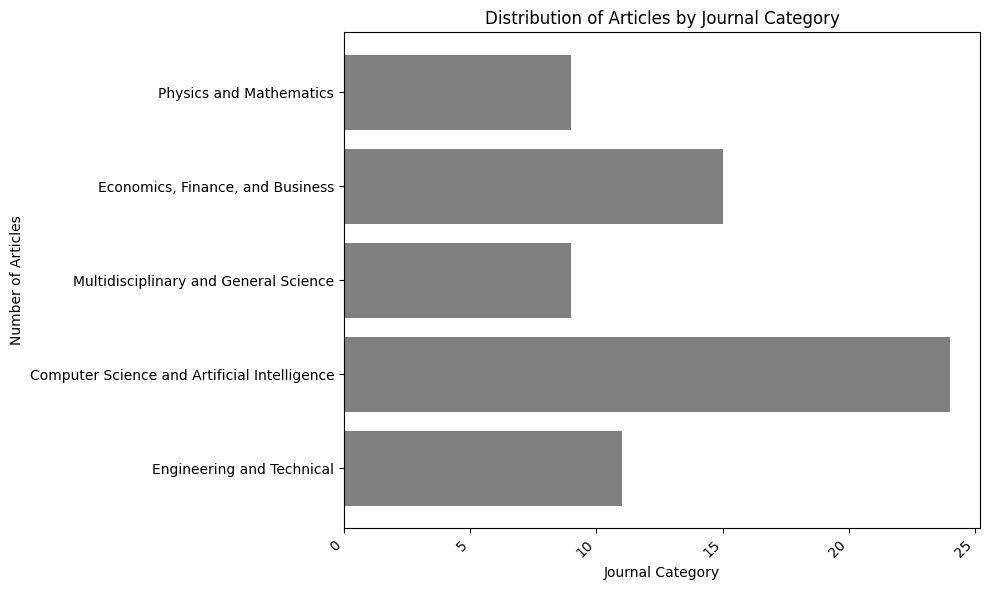
\includegraphics[width=1\linewidth]{Images/num_papers_per_journal_category.png}
    \caption{Distribution of sample papers by journal category.}
    \label{fig:num_papers_per_journal_category}
\end{figure}
%The papers in the samples explores different predictive objectives within the financial domain. As shown in Figure \ref{fig:what_is_predicted}, most papers forecast asset prices, classifications or uncertainty quantification of asset prices. [CHANGE GRAPH AFTER NEW MAPPING]
%\begin{figure}[H]
%    \centering
%    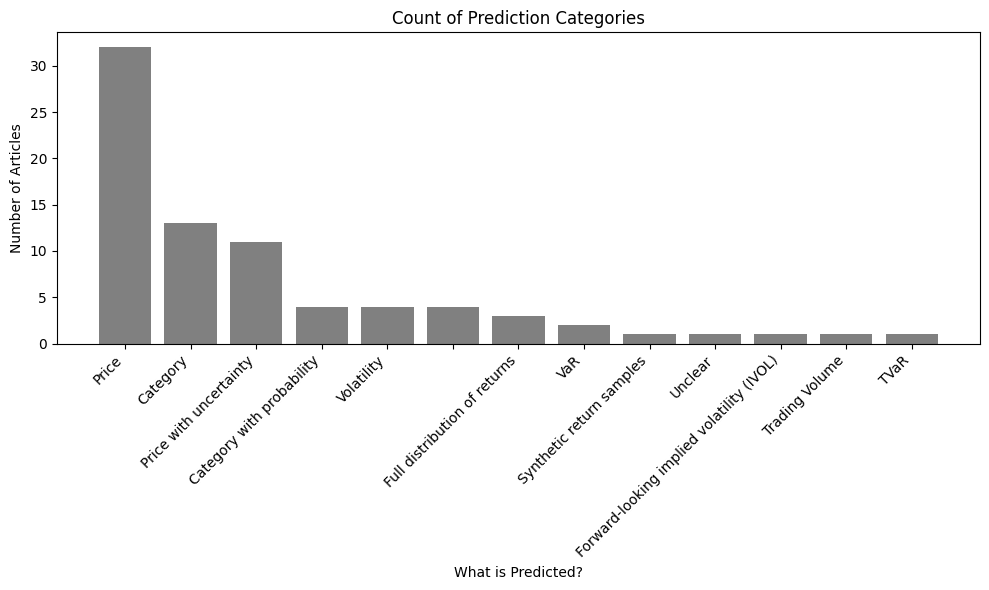
\includegraphics[width=1\linewidth]{Images/what_is_predicted.png}
%    \caption{Distribution of predictive objectives in the sample papers.}
%    \label{fig:what_is_predicted}
%\end{figure}
Figure \ref{fig:treemap_asset_by_market} illustrates the specific financial assets and markets that are focused on and forecasted in the studies. The majority of papers focus on equites, primarily stock and stock indices, but a notable number of papers also address derivatives and currencies. Each individual asset predicted in every paper is counted once.   
\begin{figure*}[h]
    \centering
    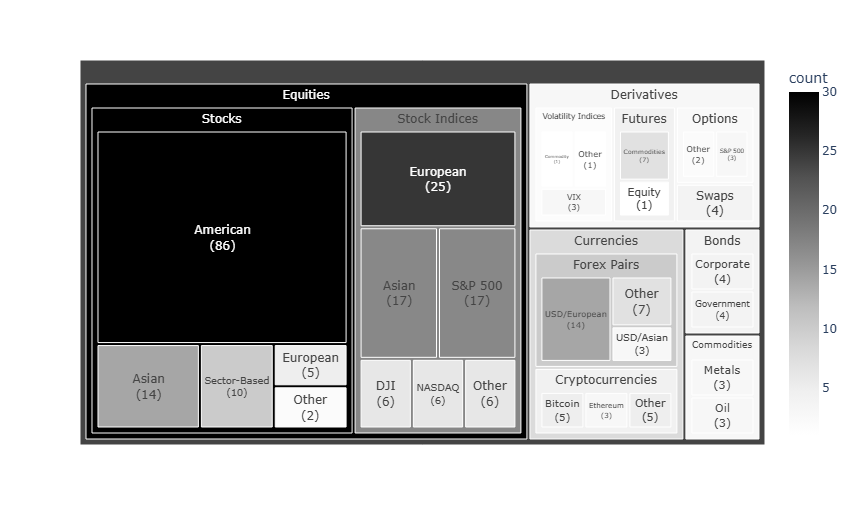
\includegraphics[width=1\linewidth]{Images/treemap_asset_by_market.png}
    \caption{Distribution of financial markets and assets targeted in the predictive models in the sample papers. \tablefootnote{Sector-Based stocks refer to Select Sector Portfolios like XLB, XLY, etc.}}
    \label{fig:treemap_asset_by_market}
\end{figure*}

Only 10 of 61 papers disclose the code for the proposed models. This lack of code disclosure can make reproducibility impossible, as the models are often too complex to enable reproduction based only on the descriptions in the articles. Additionally, it might make it more difficult for future researchers to build upon the existing research.




%----------------------------------------------------%
% --------- Analysis by Model -----------------------%
%----------------------------------------------------%

\subsection{Analysis by Model}
\label{sec:analysis_by_model}
To give an overview of the field, we present the most predominantly used probabilistic models in the sample papers, give a description of them, depict their use, and provide an overview of how they are used to create uncertainty estimates in financial time series. Table \ref{table:model_categorization} provides an overview of probabilistic model categories created based on grouping the most commonly used model types, and specifically what model names in the papers they include. Figure \ref{fig:model_breakdown} illustrates the occurrence of each probabilistic model category, and if they are used independently or in combination with other machine learning or econometric models. Summarizing results and conclusions by model type are shown in Table \ref{table:conclusions_by_model}.

\begin{table}[H]
    \centering
    \caption[Model Categorization]{Probabilistic Model Categorization}
    \label{table:model_categorization}
    \small
    \begin{adjustbox}{width=0.5\textwidth,center}
    \begin{tabular}{p{0.2\textwidth}p{0.30\textwidth}}
        \toprule
        \textbf{Model Category} & \textbf{Models} \\
        \midrule
        Bayesian Neural Networks (BNN) & BNN, Gen-BNN, B-TABL \\
        \addlinespace
        \hdashline[0.2pt/3pt]
        \addlinespace
        Gaussian Processes Regression (GPR) & GP, GPR, G4P, GPMCH \\
        \addlinespace
        \hdashline[0.2pt/3pt]
        \addlinespace
        Variational Autoencoders (VAE) & VAE \\
        \addlinespace
        \hdashline[0.2pt/3pt]
        \addlinespace
        Hidden Markov Models (HMM) & HMM, MCHMM \\
        \addlinespace
        \hdashline[0.2pt/3pt]
        \addlinespace
        Probabilistic Recurrent Neural Network (RNN) Extensions & DeepAR, DeepARA, P-GRU, QRBiLSTM, ESVM, Bayesian LSTM, Bayes ES-LSTM \\
        \addlinespace
        \hdashline[0.2pt/3pt]
        \addlinespace
        Probabilistic Generative Adversial Networks (GAN) & CGAN, PredACGAN \\
        \addlinespace
        \hdashline[0.2pt/3pt]
        \addlinespace
        Probabilistic Neural Networks (PNN) & PNN, P FF-ANN \\
        \addlinespace
        \hdashline[0.2pt/3pt]
        \addlinespace
        Other Bayesian Methods & B-SVR, BGLM, Naïve Bayes, Bayesian Network \\
        \addlinespace
        \hdashline[0.2pt/3pt]
        \addlinespace
        Other Probabilistic Methods & RSMAN, PLPR, Recurrent Dictionary Learning (RDL), TV-Entropy, Gaussian Mixture Model (GMM), IMoLSO, Fitting error analysis, Probabilistic Fuzzy Logic, Leave-One-Out Cross-Conformal Predictive System (LOO-CCPS), PSVM  \\
        \addlinespace
        \addlinespace
        \bottomrule
    \end{tabular}
    \end{adjustbox}
\end{table}

\begin{figure}[H]
    \centering
    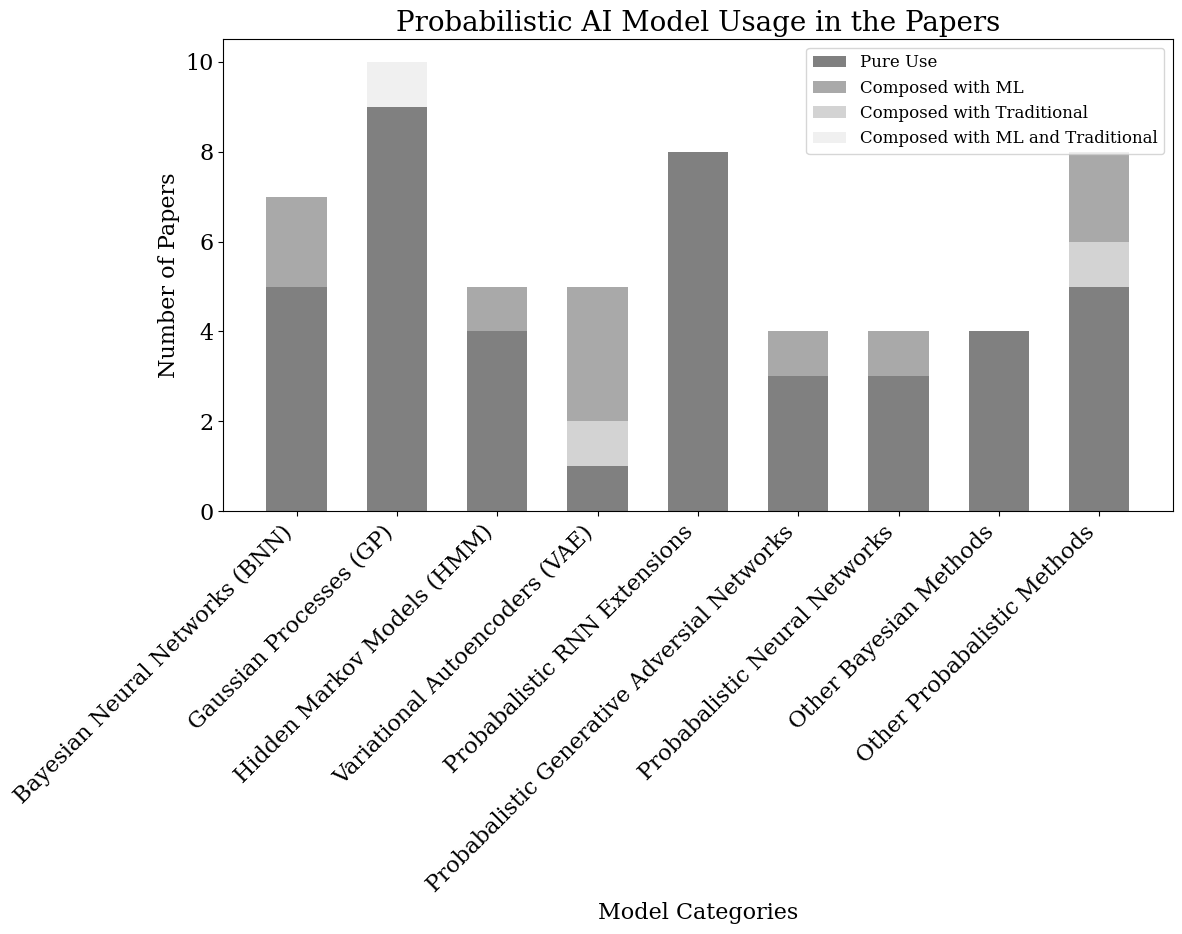
\includegraphics[width=1\linewidth]{Images/model_breakdown.png}
    \caption{Probabilistic Model Usage Breakdown}
    \label{fig:model_breakdown}
\end{figure}

%--------------------- BNN --------------------------%

\subsubsection{Bayesian Neural Networks (BNNs)}
\label{sec:bnn}

A Bayesian Neural Network (BNN) extends a traditional neural network by integrating Bayesian inference principles, allowing for the modeling of uncertainty in the network parameters \parencite{neal1995bayesian}. 
\\
\\
Conventional neural networks define a mapping from inputs $x$ to outputs $y$ using a set of trainable weights and biases $w$, represented by
\begin{equation}
    \begin{gathered}
        y = f(x;w),
    \end{gathered}
\end{equation}
where $f$ is the composition of linear transformations and non-linear activation functions across multiple layers. BNNs extend this by providing a probabilistic implementation of a standard neural network where the weights and biases are represented as random variables with probability distributions \parencite{chandra2023bayesian}, allowing the model to capture parameter uncertainty. 

Initially each weight is assigned a prior distribution
\begin{equation}
    \begin{gathered}
        p(w) = \Pi_{i} p(w_i),
    \end{gathered}
\end{equation}
where $p(w)$ represents the joint prior distribution over all weights. Combined with the likelihood of observed data $D = \{(x_n,y_n)\}_{n=1}^N$ given the weights
\begin{equation}
    \begin{gathered}    
        p(D|w) = \Pi_{n=1}^Np(y_n|x_n,w),
    \end{gathered}
\end{equation}
these form the posterior distribution over the weights using Bayes rule \parencite[p. 46]{pml1Book}
\begin{equation}
    \begin{gathered}
        p(w|D) = \frac{p(D|w)p(w)}{p(D)}.
    \end{gathered}
    \label{eq:bayes_theorem} 
\end{equation}
Predictions for new inputs $x^*$ are consequently made by integrating over the posterior distribution of the weights
\begin{equation}
    \begin{gathered}
        p(y^*|x^*,D) = \int p(y^*|x^*,w)p(w|D)dw.
    \end{gathered}
\end{equation}
By averaging over all possible weight configurations weighted by their posterior, the BNN accounts for uncertainty in parameters, resulting in a predictive distribution rather than single point estimates. This approach enables probabilistic forecasts, making them particularly suitable for uncertainty quantification \parencite{jospin2022hands}.

Both \textcite{cocco2021predictions} and \textcite{jang2018empirical} employ BNNs for cryptocurrency price predictions, primarily focusing on point estimates. \textcite{cocco2021predictions} apply a BNN with Monte Carlo approximation to predict daily Bitcoin and Ethereum prices, benchmarking against LSTM and Feed Forward Neural Networks. The BNN underperforms on Bitcoin in terms of MAPE but yields better results for Ethereum, while deployed two-stage models outperform all other. Although the authors use the BNN's outputted quantiles as prediction confidence, the authors are focused on point predictions and do not assess uncertainty. Similarly, \textcite{jang2018empirical} employ a BNN to make point predictions for Bitcoin price and volatility, using blockchain-specific data, outperforming linear regression and SVR on MAPE and RSME. The authors present confidence intervals for price and volatility, which could be used to assess total uncertainty. However, the probabilistic output is not leveraged to integrate these measures, nor is uncertainty explicitly evaluated as focus lie on point predictions. Notably, predictions frequently exceed the stated upper and lower bounds. 

\textcite{chandra2021bayesian} apply a BNN with Markov Chain Monte Carlo (MCMC) for multi-step stock price forecasting, benchmarking it against feed forward neural networks trained with ADAM and SGD. The BNN provide superior point estimates in terms of RSME for all stocks. The authors use the probabilistic output of the BNN to create prediction intervals as a measure of uncertainty. However, the quality or robustness of the estimate is not assessed, and evidently the actual stock price frequently fall outside the bounds for some stocks, indicating an unreliable uncertainty estimate. The authors do compare uncertainty levels during and after Covid, showing higher predicted uncertainty during the pandemic.

\textcite{soleymani2022longterm} propose a hybrid model, QuantumPath, combining a BNN with a temporal GAN to predict long-term prices for several S\&P 500 stocks. The BNN predicts the drift and volatility parameters for a Feynman-Dirac integral, which simulate stock trajectories by Monte Carlo, while the temporal GAN generates trajectories by condsidering the most probable paths. The probabilistic BNN output thus estimates the underlying probability distribution of the stock trajectories, and is therefore used implicitly as a volatility estimate. The models weighted expected values for 30-day predictions outperform models like GARCH, ARIMA and Ornstein-Uhlbeck. Even though the trajectories represent a distribution of prices, the total uncertainty is not assessed, and the BNN paramater estimates are not benchmarked against alternative methods.

\textcite{hortua2024forecasting} employ a BNN to forecast the VIX creating a hybrid architecture, combining WaveNet, a Temporal Convolutional Network (TCN) or  Transformers, with Bayesian inference techniques like the Reparametrization Trick (RT), Flipout and Multiplicative Normalizing Flows (MNF). The authors apply quantile recalibration to correct the miscalibration tendency in neural networks, addressing unreliable uncertainty estimates due to error overestimation, by aligning observed and expected data proportions within prediction intervals. assessed using Root Mean Squared Calibration Error (RMSCE). The models using MNF demonstrate the most reliable predictions, and generally superior short-term point predictions, outperforming traditional ARIMA. 

\textcite{magris2023bayesian} introduce a Bayesian Temporal Augmented Bilinear Network (B-TABL) for forecasting and classifying mid-price changes in Limit Order Books (LOB). Employing a Variational Online Gauss-Newton (VOGN) method for Bayesian inference, the model yield better calibrated class probabilities than approaches like Monte Carlo Dropout. Expected Calibration Error (ECE) and Expected Calibration Distance (ECD) are used to evaluate how well predicted probabilities align with actual observed frequencies, assessing model reliability in uncertainty estimation. The BNN framework provide predictive distributions for class probabilities, offering an uncertainty measure the authors interpret as confidence. While VOGN optimizer for B-TABL does not clearly outperform ADAM on standard classification metrics, the authors argue that the model deliver more meaningful classifications due to superior calibration scores. 


%--------------------- GPR ------------%

\subsubsection{Gaussian Process Regression (GPR)}
Gaussian Process Regression (GPR) is a probabilistic Bayesian model that makes no specific assumptions about the functional form of the underlying data, making it well-suited for flexible regression tasks. Much of the modern framework for Gaussian Process Regression in machine learning was formalized by \textcite{rasmussen_williams_2006}. Gaussian process is used to perform inference over functions, defining a distribution over possible functions $f(x)$ that fit the given data. Formally, a Gaussian Process (GP)  is defined as: 
\begin{equation}
f(x) \sim \mathcal{GP}(m(x), k(x, x'))
\end{equation}
where $m(x)$ is the mean function $\mathbb{E}(f)$, and $k(x, x')$ is the covariance function, also known as kernel defining how function values at point $x$ and $ x'$ effect each other:
\begin{equation}
k(x, x')=Cov(f(x),f(x'))
\end{equation}
Based on the posterior distribution, Bayesian inference (\ref{eq:bayes_theorem}) is applied to determine the most likely function $f$ that fits the data making it possible to make new predictions as new data is observed \parencite{rasmussen_williams_2006}. Since GPR provides  a predictive mean $\mathbb{E}(f_*)$ and a predictive variance $Var(f_*)$, it allows for producing predictions in addition to uncertainty estimates and confidence intervals for each prediction. GPR is therefore inherently probabilistic since it instead of only providing a single point estimate provides a distribution over predictions.  The probabilistic output consequently make GPR highly useful for modeling uncertainty in financial time series, where the degree of uncertainty often is more important than the prediction itself. 

There are 12 papers in total that use GPR. Mainly used independently, only two papers has combined it with other ML models. 

\textcite{Suphawan2022gpr} employed GPR to tackle the non-linear and non-stationary nature of the market when forecasting the Stock Exchange of Thailand (SET). The model was compared to ANN and RNN and demonstrated superior prediction accuracy on traditional error measures (RMSE, MAE, MAPE, NSE). The model allowed for providing confidence interval of the prediction results which the authors concludes makes GPR advantageous compared to ANN and RNN models.

In \textcite{Wang2021gpr} a multi-scale nonlinear ensemble model incorporates GPR to predict stock indices for S\&P 500, Dow Jones and NASDAQ. The ensemble model use Variational Mode Decomposition (VDM) and an Auto-Encoder (AE) for feature extraction, and a two-step deep learning setup with RNN and LSTM. GPR plays a critical role in the final stage to create interval prediction and uncertainty estimates. The model is benchmarked against a regular GPR and other machine learning models such as ANN, RNN and LSTM, displaying improvements in MAPE, MSE, RMSE, MAE and SSE for point predictions. In addition the interval prediction are assessed on coverage probability metrics like Mean Width Percentage (MWP), Mean Coverage (MC) and Prediction Interval Coverage Probability (PICP) which shows better results than GPR alone. In another paper by the same authors, \textcite{Wang2021gprensemble} presents an alternative ensemble (SSA-EWSVM-RNN-GPR) for stock index forecasting using Singular Spectrum Analysis (SSA) and Enhanced Weighted Support Vector Machine (EWSVM) for interval prediction, which is then further processed by an RNN before GPR is used to provide interval forecasts. MWP and CP were used to validate the GPR-based interval forecast and the model showed improved point accuracy forecasting and uncertainty estimate compared to eight GPR benchmark models.  

\textcite{Li2024gpr} integrated a GPR model into a graph-aware portfolio selection model with Generalized Gaussian Distribution (GGD) likelihood capturing both return mean and variance. The GPR model-based portfolio performed better than traditional mean-variance methods, but is outperformed by amongst other Uniform Constant Rebalanced Portfolio (UCRP).

\textcite{Platanios2014gpr} adopted a GPR model into a Gaussian Process Mixture Conditional Heteroscedasticity (GPMCH) model to forecast price and financial volatility for currency exchange rates and global large-cap equity indices. The model captures volatility clustering and handle the non-linear dependency, presenting a viable alterative to traditional GARCH models. The authors applies a Pitman-Yor process to better capture skewed and tail heavy data distributions, and showed that their GPMCH outperformed GARCH in volatility predictions.

In \textcite{tegner2021probabilistic}, Gaussian Process Regression (GPR) is used to transform market option price data into a smooth implied volatility surface, capturing implied volatility across various strike prices and maturities. GPR is then applied to forecast future values of this surface, enabling predictions of implied volatility and, consequently, future option prices. The results indicate a promising ability to forecast the VIX one week ahead, outperforming a naive forecasting approach, but no other benchmark models are considered.

Estimation of portfolio tail risk, specifically VaR and TVaR, has seen accuracy improvement with GPR models as demonstrated by \textcite{Risk2018gpr}. The model's spatial modeling enabled efficient risk estimations across simulated economic scenarios with Monte Carlo simulations. Bias and variance in the risk estimates was reduced compared to traditional nested simulations and methods. The authors use the model to distinguish between epistemic and aleatoric uncertainty. In one of the advanced models the authors present, they use heteroskedastic GP (hetGP), which allowed for handling scenarios of varying levels of noise more effectively, further enhancing the uncertainty estimates. 

The last studies in the sample utilizing GPR--\textcite{Papaioannou2022gpr}, \textcite{Zmuk2020gpr}, \textcite{Park2014gpr}, and ~\textcite{DeSpiegeleer2018gpr}--apply GPR for price prediction in financial time series and \textcite{Hocht2024gpr} predict forward-looking implied volatility (IVOL), generally demonstrate competitive performance against traditional models. However, these works focus primarily on point predictions without assessing the probabilistic outputs of the GPR model or quantifying prediction uncertainty.




%--------------------- VAE --------------------------%


\subsubsection{Variational Autoencoders (VAEs)}
Variational Autoencoders (VAEs) are generative models that combine principles from deep learning and variational inference to learn probabilistic representations of data. Introduced by \textcite{kingma2013auto} as Auto-Encoding Variational Bayes, the model architecture distinguishes itself from traditional autoencoders by utilizing stochastic elements in the two main components: the encoding and decoding processes. 
\\
\\The encoder maps input vector data $x$ to a latent space $z$, producing the parameters (mean and variance) of a probability distribution $q_\phi(z|x)$ over the latent variables, where $\phi$ denotes the parameters of the encoder network. The decoder subsequently reconstructs the original input data from this latent representation by mapping samples $z \sim q_\phi(z|x)$ through $p_{\theta}(x|z)$ aiming to model the true distribution
\begin{equation}
    \begin{gathered}
        p_\theta(x) = \int p_\theta(x|z)p(z)dz,
    \end{gathered}
\end{equation}
where the decoder is parameterized by $\theta$. However, due to intractable computation of the exact posterior $p_{\theta}(z|x) = \frac{p_{\theta}(x|z) p_{\theta}(z)}{p_{\theta}(x)}$, variational inference over the latent variables is employed to approximate it with $q_\phi(z|x)$ \parencite{kingma2013auto}. As the encoder outputs a distribution over the latent variables, uncertainty can be captured in the latent representation by drawing multiple samples. These samples can then be propagated through the decoder, ultimately resulting in a distribution of reconstructed outputs. 


Only one article in the sample uses a VAE independently. \textcite{arian2022encoded} propose Encoded VaR, directly applying VAE to estimate VaR by generating synthetic market scenarios from historical cross-sectional stock returns of the S\&P 500, LSE and FSE. The VAE learns the latent structure of the financial return distributions without relying on parametric assumptions or predefined joint distributions, and in turn generating samples of synthetic returns to be interpreted as potential future outcomes. The VAE architecture allows generation of arbitrarily many samples, allowing the reconstruction a theoretical underlying distribution for VaR calculation. The authors claim to enhance the signal-to-noise ratio present in financial data, and benchmark against traditional GARCH models. While the model shows competitive results for specific loss functions like Lopez' method \parencite{lopez1998methods}, GARCH extensions (CaViaR-GARCH and EVT-GARCH) generally perform equally well and yield statistically significant p-values across all adequacy tests, in contrast to the Encoded VaR. 

Of the papers utilizing VAEs in combination with other models, several use it as a probabilistic input to another model and do not directly infer uncertainty estimates from the probabilistic output of the VAE.  
\textcite{caprioli2023quantifying} extend the use of VAEs for risk management to assess credit portfolio sensitivity to asset correlations. The VAE is used to generate synthetic correlation matrices, simulating various market conditions, used as input in a multi-factor Vasciek model with Monte Carlo simulation to examine how shifts in correlations affect VaR. \textcite{choudhury2020enhancing} use VAEs as a pre-processing tool to denoise NASDAQ stock financial time series before using a stacked LSTM autoencoder to make point predictions. The authors report superior results in point predictions compared to other machine learning models like, but do not assess uncertainty in their forecasts.  \textcite{tang2024period} also uses VAEs for denoising financial time data by extracting latent representations. The model is combined with a transformer (LPAST), and is used for long-term multi-step point predictions of different financial times series. The proposed method outperforms compared machine learning models in point predictions, but again the probabilistic outputs of the VAE are not directly utilized for distributional forecasts or for uncertainty quantification. \textcite{li2020multivariate} combine a multimodal VAE with a LSTM architecture to predict agriculture commodity futures. The VAE is used to extract high-level features and reduce noise for input data in the LSTM, and probabilistic output is not used specifically in predictions. Their proposed model outperforms traditional econometric models like ARIMA, and other machine learning benchmarks like CNNs. 

\textcite{xing2019sentiment} propose an innovative approach by combining VAEs with a RNN to forecast stock volatility. Their model, Sentiment-Aware Volatility Forecasting (SAVING), integrates social media sentiment data to jointly model stock price movements and the sentiment that influences them. This interaction is captured through the VAE's latent variables, from which marginal joint probabilities are inferred. Benchmarked against econometric models GARCH, EGARCH and TARCH using negative log-likelihood, the SAVING model demonstrate superior performance in terms of negative log-likelihood (NLL).

%--------------------- HMMs --------------------------%

\subsubsection{Hidden Markov Models (HMMs)}
Hidden Markov Models (HMMs) are probabilistic models used to analyze sequential data with underlying unobservable structures \parencite{rabiner1986introduction}, building on Markov chain theory. In finance, HMMs can therefore be applied to model time series where market states, such as bull or bear markets, periods of low or high volatility, or other economic regimes, are not directly observable. 

The classic HMM consists of a finite set of hidden states $S = \{s_1, s_2, ... s_N\}$ and a corresponding set of observable outputs $O = \{o_1, o_2, ... o_T\}$. The model is defined by an initial probability distribution $\pi_i = P(q_1 = s_i)$, state transition probabilities $a_{ij} = P(q_{t+1} = s_j|q_t = s_i)$ and the emission probabilities specifying the likelihood of observations given system state $b_j(o_t) = P(o_t|q_t=s_j)$. Consequently, HMMs are capable of producing distributional forecasts by utilizing the predictive probability distribution of future observations
\begin{equation}
        P(o_{T+1}|O) = \sum_{i=1}^{N}P(o_{T+1}|q_{T+1} = s_i)P(q_{T+1} = s_i | O).
\end{equation}
The probabilistic modeling of both hidden states and observations allow for the computation of confidence intervals and prediction reliability, thereby facilitating uncertainty estimation of predictions. 

Two articles in the final sample use HMMs to address multi-factor dependencies in financial time series forecasting. \textcite{li2010stochastic} propose a stochastic HMM for forecasting fuzzy time series data, modeling the Taiwan Weighted Stock Index as the hidden states and the New Taiwan dollar against the U.S. dollar as the observable state. While the model performs better compared to a standard HMM implementation in forecasting accuracy, it is not evaluated against any other models. Additionally, they focus solely on point predictions, without assessing the probabilistic output of their model. \textcite{cao2019multi} extend the multi-factor dependency approach by developing a Multi-Layer Coupled HMM (MCHMM). Unlike \textcite{li2010stochastic} who address dependencies within a single market, \textcite{cao2019multi} capture interactions both within and between markets, specifically between stock and currency markets across different countries. The authors experiment predicting categorical trends of German and Dutch stock markets, reporting better accuracy than traditional models like ARIMA and logistic regression. However, similar to \textcite{li2010stochastic}, they  do not assess uncertainty in predictions that can be derived from the probabilistic output of the model.

In \textcite{park2011trend}, historical segments of financial time series are labeled as either up-trending or down-trending using the Perceptually Important Points (PIP) algorithm. Continuous Hidden Markov Models (HMMs) are then trained to classify out-of-sample data. The results demonstrate that the HMM-based model significantly outperforms Support Vector Machines (SVMs) across most tested assets, including currencies, stock indices, and individual stocks.

\textcite{sher2023exploiting} also focus on forecasting categorical return trends, applying HMM alongside several other models to forecast movements in individual technology stocks. Although the details around their specific model implementation are limited, the authors report superior performance from the HMM compared to ARIMA, LSTM and several booster models. The probabilistic output of HMM is leveraged to assess the likelihood of future stock price movement, but like the previous studies, uncertainty assessment is not addressed. 

\textcite{zhang2019high} extend the HMM to a second-order model, capturing both short-term and long-term dependencies for predicting next-day categorical trends in stock indices. In their higher order approach, the observation depends not only on the current state, but also on the previous $m-1$ hidden states. While the authors do not directly use the probabilistic distribution output to assess uncertainty, they suggest that the higher-order HMM has lower risk then the first-order model, supported by improved Sharpe ratios and reduced maximum drawdown in their trading strategy experiment. Additionally, the second-order HMM deliver better predictive performance compared to the first-order HMM.

Similarly, \textcite{su2022hmm} applies the second-order HMM model to predict prices and directions of the Hang Seng Index (HSI). Even though their model is capable of producing distributional forecasts, the authors focus exclusively on point predictions and do not assess uncertainty of any kind. When compared to models like NA-GARCH, CNN-BiLSTM-AM and AHMMAS, the second-order HMM showcases superior performance. 


%--------------------- Prob RNN extensions --------------------------%


\subsubsection{Probabilistic RNN Extensions}
\label{sec:prob_rnn}

Probabilistic extensions of Recurrent Neural Networks (RNNs) refer to models augmenting standard RNN implmentations with stochastic components, enabling them to generate probabilistic forecasts. RNNs are neural networks designed to handle sequential data by maintaining hidden states that capture information about previous inputs to shape subsequent behavior \parencite{Elman1990Finding}, making them suitable for financial time series analysis. In a standard RNN the hidden state $h_t$ at time step $t$ is updated based on the current input $x_t$ and the previous hidden state $h_{t-1}$:
\begin{equation}
    \begin{gathered}
        h_t = \phi(W_{xh}x_t + W_{hh}h_{t-1} + b_h)
    \end{gathered}
\end{equation}
where $\phi$ is an activation function, $W_{xh}$ and $W_{hh}$ are weight matrices and $b_h$ is a bias vector. 

Standard RNNs suffer from the exploding and vanishing gradient problems \parencite{Pascanu2013Difficulty}, which hinder long-term dependencies and make training difficult. To address this issue, advanced architectures like Long Short-Term Memory (LSTM) networks \parencite{Hochreiter1997LSTM} and Gated Recurrent Units (GRU) \parencite{Cho2014Learning} have been introduced, incorporating gating mechanisms to control the information flow. 

Several articles apply Bayesian methods within RNN implementations, placing prior distribution over the network weights to estimate the posterior distribution (Equation \ref{eq:bayes_theorem}). \textcite{Hassan2024Bitcoin} utilize a Bayesian LSTM with MC dropout at inference, optimized with ADAM, to generate a distributional forecast of Bitcoin prices. The model outperforms non-Bayesian LSTMs in RMSE, $R^2$ and MAPE for point predictions, and the Bayesian approach facilitate model uncertainty quantification. The author argues that the model uncertainty is accurately estimated, as it increases with prediction distance from actual data, but no other assessment measure of the quality of the uncertainty estimate is utilized. Similarly, \textcite{Dixon2022Industrial} incorporate exponential smoothing within a Bayesian RNN, smoothing hidden states to capture long-term dependencies in IBM stock predictions. The model provide more accurate forecasts compared to a standard LSTM and GRU implementation, with better coverage of confidence intervals across various predictive horizons. This improvement is presented as evidence of superior uncertainty estimation, though no distinction between model uncertainty and aleatoric uncertainty is made.

\textcite{Parker2021BayesianHeteroskedastic} present a Bayesian general heteroskedacity model (GBHM) within an RNN framework to predict Dow Jones index volatility. Compared to a GARCH implementation, the model achieves superior log predictive scores. Additionally, the authors report more accurate uncertainty measured by coverage, with GARCH yielding an inflated 100\% coverage for the 50\% prediction interval, while the model attains nearly optimal 50\%. Previous research has shown that GARCH generally produces reliable coverage probabilities when modeling stock indices \parencite{Rippel2011ValueAR}, so this result raises questions about whether the GARCH model they have benchmarked against is misspecified.

\textcite{Tian2023} forecast volatility indices using a Clockwork RNN optimized with a Cuckoo-Search-enhanced multi-objective grey wolf optimizer, employing empirical mode decomposition to capture both linear and nonlinear trends. The model produces deterministic and probabilistic forecasts, with uncertainty quantified and distinguished using PICP, PINAW, and Winkler score. It demonstrates superior accuracy and stability across case studies, including the VIX, crude oil ETF volatility index (COEVI), and the 10-year U.S. treasury note volatility index (TYVIX).

\textcite{Golnari2024Cryptocurrency} introduce a probabilistic GRU model incorporating Bayesian inference to treat network weights as probabilistic, enabling distributional forecasts
 for crypto price predictions. The model outperforms traditional LSTM and GRU implementations in MAPE and $R^2$ of point predictions. The authors use the standard deviation of the forecast distributions as a measure of prediction uncertainty, but do not further assess it's reliability or distinguish uncertainty types.  

\textcite{Wang2024GoldForecasting} employ Quantile Regression (QR) within a Bi-Directional LSTM model to produce probabilistic range predictions for gold prices, incorporating several macroeconomic factors. The QR-BiLSTM predicts multiple quantiles of the future price distribution, capturing price fluctuations and is used as a measure of uncertainty. The authors assess the total uncertainty of the predicted distributions, without separating model and underlying uncertainty, using the Average Internal Score (AIS), which balances interval width and accuracy. This evaluation demonstrate that their model outperform other LSTM and GRU benchmarks. 

Three articles in the sample employ the DeepAR model \parencite{Salinas2019DeepAR}, an autoregressive RNN-based model that generate parameters of a predefined probability distribution at each time step. \textcite{Fatouros2023DeepVaR} apply DeepAR to forecast VaR for a forex portfolio, comparing it to GARCH and other models using Christoffer's and Dynamic Quantile tests for adequacy. Their results are promising as the adequacy tests are passed, with superior accuracy in most loss functions. \textcite{Almeida2024RiskForecasting} use DeepAR to forecast VaR and ES for crypto liquidity pool portfolios, reporting superior accuracy in ES prediction over GARCH. However, without any adequacy tests, interpretation of results is unvalid. \textcite{Li2024DeepAR} extend DeepAR with an attention mechanism (DeepARA) for stock price forecasting in the Chinese market, achieving superior MAPE in point predictions compared to other neural networks. The authors assess uncertainty by analyzing the entropy of the predicted price distributions concluding that the model provide good estimates, but lack comparative uncertainty evaluation, as no alternative models considered provided comparable distributions.  

%---------------------  P GANs --------------------------%


\subsubsection{Probabilistic Generative Adversarial Networks}
Generative Adversarial Networks (GANs) are a class of deep learning models that was introduced by \textcite{goodfellow2014gan}, providing a framework for estimating generative models though adversarial process \parencite{goodfellow2014gan}. GANs consist of two neural networks, a generator $G$ and a discriminator $D$ that are trained in a two-player competitive minimax game.
The generator produce synthetic data that aims be as close to real data as possible, while the discriminator tries to distinguish between synthetic and real data samples. Both networks iteratively try to improve. 

The probabilistic capabilities of GANs comes from the generators ability to map random noise $p_z(z)$, like for example Gaussian, to a probability distribution of outputs similar to the real data distribution $p_{\text{data}}(x)$ enabling it it capture the uncertainty in real-world-data. The objective can formally be formulated as: 
\begin{equation}
\min_{G} \max_{D}  \mathbb{E}_{x \sim p_{\text{data}}(x)}[\log D(x)] + \mathbb{E}_{z \sim p_z(z)}[\log (1 - D(G(z)))]
\end{equation} 

Four articles in the sample used GANs in their financial forecasting. For example, \textcite{lee2021estimation} proposed a modified conditional GAN (cGAN-UC) as a probabilistic model to forecast the price of NASDAQ-100 Future Index with uncertainty. The authors used the generator to predict rather than for sample generation to be used as a probabilistic predictive neural network. The cGAN model outperformed traditional deterministic models such as Artificial Neural Networks (ANNs), Random Forest, Ridge and Lasso regression, and probabilistic models like Bayesian Neural Networks (BNNs) for both point accuracy and uncertainty estimation especially in noisy data due to the benefits of adversarial training. 

\textcite{vuletic2024finGAN} introduced a specialized GAN model (Fin-GAN) for one-step-ahead probabilistic prediction of stock and stock indices price with uncertainty. The model uses a cGAN architecture with an economics-driven loss function, to enhance Sharpe Ratio and integrate risk directly in the model. The model outputs a full conditional probability distribution of returns witch allows it to estimate the financial uncertainty. The Fin-GAN model claims to outperform and achieve higher Sharpe Ratio compared to traditional time-series modes such as ARIMA and LSTM, and allows for uncertainty informed portfolio allocation due to its probabilistic outputs. However, the paper does not compare the uncertainty estimation against other probabilistic or ML models. 

For portfolio optimization, \textcite{kim2023portfolio} applies a predictive auxiliary classifier GAN (PredACGAN) on S\&P 500 and NASDAQ 100 stocks. The generator forecasts future returns based on historical data and produce distributions reflecting prediction uncertainty. The authors construct a portfolio based on the predictions, where they combine the expected return with the distribution's entropy as a risk measure to maximize risk-adjusted returns. The PredACGAN portfolio resulted in higher Sharpe Ratio and lower maximum drawdown in comparison to traditional risk-agnostic portfolios and other ML models (e.g. Ridge classifiers and gradient boosting).

\textcite{salama2024gan} applies a similar approach using a cGAN model but aims to increase performance by integrating a spotted hyena optimization algorithm with a GAN for time series forecasting (SHOAGAI-TSF) technique. The Spotted Hyena Optimization Algorithm (SHOA) optimize the model's hyperparameters to enhance prediction accuracy. The integration improves Mean Absolute Error (MAE) and Mean Squared Error (MSE) performance compared to other GAN-based model, however even though the model provides full probabilistic distribution, the paper does not use it to asses uncertainty but focus on improving prediction accuracy. 


%--------------------- PNNs --------------------------%

\subsubsection{Probabilistic Neural Networks (PNNs)}
Probabilistic Neural Networks (PNNs) are a class of feedforward neural networks with four layers leveraging statistical principles mainly for classification tasks. First introduced by \textcite{Specht1990pnn}, it builds on Bayesian decision theory in order to estimate full probability distribution for the cases given the input \parencite{Specht1990pnn}. PNNs are inherently probabilistic as they utilize probability density functions (PDF) to create output based on posterior probabilities making it possible for confidence assessment of the classifications. The class-conditional probability for an input $x$ is given by:
\begin{equation}
P(x \mid C_i) = \frac{1}{N_i} \sum_{j=1}^{N_i} \exp \left( -\frac{\| x - x_j \|^2}{2\sigma^2} \right)
\end{equation}
where $x_j$ are samples from $C_i$, $N_i$ number of samples in class $C_i$ and $\sigma$ is a smoothing factor. 
The probabilistic structure makes it possible for dynamic probability estimations based on new data and suitable for real-time assessment and decision-making with confidence levels for classification. 

Four papers in the sample apply PNNs.
\textcite{Thawornwong2004pnn} utilized a PNN model to predict the directions of future
excess stock return for S\&P 500 stock portfolio, where they investigate adaptive selection of economic variables for prediction by using recent relevant variables. The model demonstrates an ability to outperform traditional models such as linear regression, random walk model and neural network with constant variables. However, the model focus on directional accuracy and risk-adjusted profits to provide an alternative to the buy-and-hold strategy with reduced risk and increased profitability, rather than uncertainty quantification assessment.  

\textcite{Chandrasekara2019pnn} enhance the traditional PNN using a multivariate t-distribution instead of a Gaussian assumption. The multivariate approach makes it possible to capture the relationships between the assets. In addition they proposed a solution for addressing multi-class imbalance to prevent biased directional predictions. The model was tested on three stock market indices (AORD, GSPC, API). The proposed model with a scaled t-distribution and the multi-class undersampling based bagging (MCUB) ensemble method showed better performance and accuracy than standard PNN models independently and together in directional forecasting, although the paper does not explicitly focus on uncertainty quantification.  

\textcite{Maniatopoulos2022pnn} propose a probabilistic feed-forward artificial network (Probabilistic FF-ANN) to predict category with probability for company stocks in US Down Jones. The proposed solution builds on the PNN framework with probabilistic recovery to enhance predictive accuracy across time horizons integrated. The authors claim the Probabilistic FF-ANN outperforms CNN, FFNN, LSTM and GAN models, and are able to give 60\% future movements accuracy and a reported 60\% annual return on investment. 

\textcite{Lahmiri2024pnn} compares a PNN with a Back-Propagation Neural Network that is optimized using Genetic algorithms (GA-BPNN) for prediction daily trends in tech stocks and the NYSE index. Their results show that GA-BPNN outperforms the traditional PNN in accuracy. Although the study shows that PNN effectively leverages the probabilistic output for classification, it does not assess the accuracy of the uncertainty estimates.

%--------------------- Other Bayesian methods -----------------------%

\subsubsection{Other Bayesian methods}
Other Bayesian Methods refer to models that apply Bayesian techniques and are able to construct probability distributions to quantify uncertainty, without utilizing Bayesian inference in Neural network architectures. Rather than delving into the technical implementations of each model, we will focus on summarizing the key results they achieve. 

\textcite{Malagrino2018Forecasting} utilize a ``Bayesian network'' to predict the directional movements of the Brazilian iBOVESPA index by incorporating dependencies among multiple global stock indices, achieving competitive accuracy with comparable literature. The authors classify binary without explicitly quantifying uncertainty in classification outcomes. Similarly, \textcite{Raúl_PlazaCasado_PradoRomán_2021} apply a Bayesian network to forecast IBEX index trends, incorporating investor sentiment to enhance model performance. Here, the authors interpret the classification probabilities as trust levels that indicate degrees of uncertainty, and develop a trading system shown to systematically outperform the market.

\textcite{Grudniewicz2023Application} evaluate a Bayesian Generalized Linear Model (BGLM) alongside traditional and machine learning models for classifying stock movements to generate trading signals across various indices for algorithmic trading. Their findings indicate that algorithmic trading outperformed passive strategies, with the BGLM was among the most accurate models. However, the probabilistic output of the BGLM is not use to assess uncertainty, nor integrated into the trading strategies. 

A distinct application is proposed by \textcite{Law2017Practical}, using a Bayesian Support Vector Regression (B-SVR) for price prediction and prediction uncertainty estimates for various financial time series classes, including equity indices, commodity futures and bond yields. The Bayesian framework optimize model parameters, and the complete model produce interval predictions. The authors evaluate the uncertainty estimate quality by examining the correlation between prediction uncertainty and actual errors using the Coefficient of Variation (CoV), classifying predictions as reliable or unreliable based on a continuously calibrated threshold value, excluding unreliable predictions. The model is not benchmarked against traditional or ML models. 

%--------------------- Other probabilistic methods --------------------------%

\subsubsection{Other Probabilistic Methods}
Other Probabilistic models refer to methods capable of producing probabilistic forecasts, but do not fit easily in any of the aforementioned categories. We will present a short summary of some of the 9 articles in the category and what results they report, but will not delve into technicalities in this section. Descriptions of the rest can be found in the full table in Appendix \ref{appendix:descriptive_table_of_all_articles}. 

\textcite{Daniali2021} employ a Deep Convolutional Neural Network (DCNN) to forecast the VIX, integrating a conditional variance model in the final layer to jointly predict mean and variance. The variance is embedded within the probability-based loss function as a way to reduce uncertainty. Compared to a standard DCNN, the model demonstrated reduced error in point predictions. 

\textcite{Horenko2020} propose a multivariate nonparametric regime-switching model (TV-Entropy) based on the maximum entropy principle, applying it to forecast stock indices and estimate VaR. Compared to GARCH, TV-Entropy achieves superior Bayesian Information Criterion (BIC) scores, and better calibrated unconditional coverage on 95 and 99\% confidence intervals. 

\textcite{Sharma2021} introduce Recurrent Dictionary Learning (RDL), which incorporates the Kalman filter with smoothing algorithms to generate distributional forecasts for stocks. The model outperforms LSTM, CNN, and ARIMA in both point forecasts and next-day trend classification, while no explicit assessment of uncertainty is conducted.

\cite{wang2020fastconformal} propose a Leave-One-Out Cross-Conformal Predictive System (LOO-CCPS) combined with Regularized Extreme Learning Machine (RELM) to produce cumulative distribution functions (CDFs) for different assets. The model facilitates uncertainty estimation through prediction intervals derived from quantiles. The authors validate the model by evaluating the frequency of which values fall within the predicted quantiles, achieving superior performance compared to benchmark systems. 

The four omitted articles either employ similar models to those discussed, lack discussion of uncertainty, or use probabilistic outputs solely as inputs for point prediction models.





%---------------------Conclusion----------------------%
\subsubsection{Conclusion} % deside if we need this
Table \ref{table:conclusions_by_model} summarize conclutions by model type.

\begin{table}[H]
    \centering
    \caption[Summarizing conclusions by model type]{Summarizing conclusions by model type}
    \label{table:conclusions_by_model}
    \small
    \begin{adjustbox}{width=0.5\textwidth,center}
    \begin{tabular}{p{0.1\textwidth}p{0.4\textwidth}}
        \toprule
        \textbf{Model Category} & \textbf{Conclusion} \\
        \midrule
        Bayesian Neural Networks (BNN) & 
        \smallbullet{Primarily focused on point predictions over uncertainty estimation}
        \smallbullet{Competitive predictive performance across assets, comparable to traditional models like ARIMA and other neural networks} 
        \smallbullet{Commonly used in hybrid models (e.g. with GANs or TCNs)}
        \smallbullet{Monte Carlo is the most popular inference method, with advance techniques like MNF demonstrating promising results} \\
        \addlinespace
        \hdashline[0.2pt/3pt]
        \addlinespace
        Gaussian Processes (GP) & 
        \smallbullet{Known for reliable uncertainty estimation, often outperforms ANN and RNN}
        \smallbullet{Often used in ensemble models to enhance prediction intervals} \\
        \addlinespace
        \hdashline[0.2pt/3pt]
        \addlinespace
        Variational Autoencoders (VAE) & 
        \smallbullet{Primarily used with other models for denoising and feature extraction} 
        \smallbullet{Promising, but few papers use probabilistic output directly for uncertainty quantification} \\
        \addlinespace
        \hdashline[0.2pt/3pt]
        \addlinespace
        Hidden Markov Models (HMM) & 
        \smallbullet{Mostly used and effective for categorical predictions, outperforming traditional models} 
        \smallbullet{Minimal focus on leveraging distributional forecasts for uncertainty estimation}
        \smallbullet{Second-order HMMs show promising results but lack comprehensive benchmarking}\\
        \addlinespace
        \hdashline[0.2pt/3pt]
        \addlinespace
        Probabilistic RNN Extensions & 
        \smallbullet{Promising in recent studies with good point prediction results - most articles from 2023 and 2024} 
       \smallbullet{DeepAR manages to pass Christoffersen's test and is shown to beat GARCH at VaR estimation in one article} \\
        \addlinespace
        \hdashline[0.2pt/3pt]
        \addlinespace
        Probabilistic Generative Adversarial Networks (GAN) & 
        \smallbullet{Effective in probabilistic forecasting with cGAN models showing high potential} 
        \smallbullet{Typically outperforms traditional models, though comparisons to ML models are limited} \\
        \addlinespace
        \hdashline[0.2pt/3pt]
        \addlinespace
        Probabilistic Neural Networks (PNN) & 
        \smallbullet{Primarily focused on classification, with reliable probabilistic outputs} 
        \smallbullet{Limited emphasis on uncertainty quantification despite probabilistic architecture} \\
        \addlinespace
        \hdashline[0.2pt/3pt]
        \addlinespace
        Other Bayesian Methods & 
        \smallbullet{Strong for classification tasks, often effective in stock movement predictions} 
        \smallbullet{Typically does not leverage probabilistic outputs for detailed uncertainty analysis} 
        \smallbullet{Lacking benchmarking to other models make it hard to quantify the exact promise of the models}\\
        \addlinespace
        \hdashline[0.2pt/3pt]
        \addlinespace
        Other Probabilistic Methods & 
        \smallbullet{Diverse models with strong performance in specific applications (e.g., TV-Entropy for VaR)} 
        \smallbullet{Uncertainty rarely assessed explicitly, often focused on enhancing point accuracy} \\
        \addlinespace
        \bottomrule
    \end{tabular}
    \end{adjustbox}
\end{table}




%----------------------------------------------------%
% --------- Analysis by Target Variable -------------%
%----------------------------------------------------%


\subsection{Analysis by Model Output}
\label{sec:analysis_by_model_output}
To enhance the understanding of probabilistic AI applications in financial time series forecasting, this section categorizes the sample based on what the model outputs. While the majority of models in the sample focus on predicting returns or prices, often incorporating uncertainty estimates, some studies use volatility or volatility proxies as target variables. Figure \ref{fig:model_output} shows a breakdown of all articles in the sample by model output. Summarizing results and conclusions by model output are shown in Table \ref{table:conclusions_by_target_variable}.

\begin{figure}[H]
    \centering
    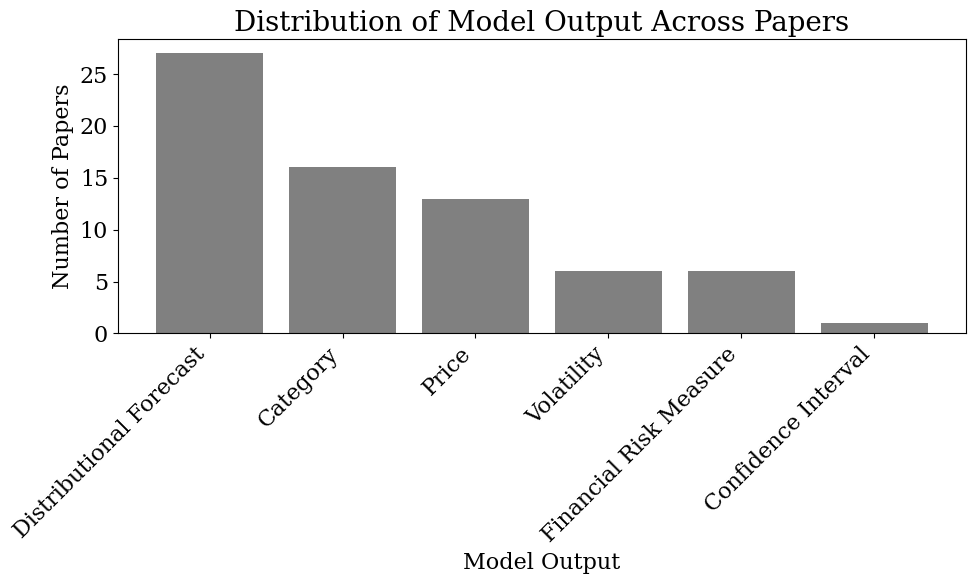
\includegraphics[width=1\linewidth]{Images/model_output.png}
    \caption{Distribution of model output categories that the models in the papers provide, note that some papers provide multiple outputs }
    \label{fig:model_output}
\end{figure}

\subsubsection{Price}
13 articles in the sample employ probabilistic AI models to predict asset prices or returns without estimating uncertainty, focusing solely on enhancing predictive accuracy. Despite using probabilistic models, these studies do not exploit their inherent capability to quantify uncertainty.

\textcite{jang2018generative} adopt a Bayesian approach to incorporate prior knowledge about option prices, specifically encoding in the prior that forecasted prices of deep in-the-money (ITM) or out-of-the-money (OTM) options should remain close to their previous prices. Thus, they are able to make better point predictions in situations that differ significantly from the training data, but they do not use the uncertainty estimates.

In \textcite{jang2018empirical}, they use a Bayesian neural network for improved regularization and generalization, outperforming linear regression and Support Vector Regression models for bitcoin price prediction.\footnote{From their model description, it is unclear if the proposed model is actually a Bayesian neural network or if they have confused the term with Bayesian regularized networks or L2-regularized neural networks.}

\textcite{choudhury2020enhancing} and \textcite{tang2024period} use Variational Auto-Encoders (VAEs) as a preprocessing step for LSTM and transformer models, respectively, which in turn generates point predictions for stock prices. The idea is that by first mapping the input to a lower-dimensional latent space, noise can be reduced, making the regression task easier. \textcite{choudhury2020enhancing} do not mention why a VAE was preferred over a conventional Auto-Encoder (AE). \textcite{tang2024period} suggest that VAEs perform better than AEs for noisy data, but neither their study nor the articles they cite empirically benchmark VAEs against AEs.

In \textcite{Sharma2021}, a clear motivation for the chosen Recurrent Dictionary Learning (RDL) structure is its ability to make predictions with uncertainty, and they mention that a knowledgeable trader can use the uncertainty estimates to make better trading decisions. However, they do not present or analyze the produced uncertainty estimates, and there is no evaluation of whether the uncertainty estimates are useful.

\textcite{Daniali2021} combine a CNN model with a conditional variance layer. The probabilistic output is not used, but the results show that the proposed model outperforms a traditional CNN in terms of point predictions.

In \textcite{govindasamy2014prediction, li2010stochastic}, predicted probabilities for different states are used to estimate a predicted price without any uncertainty quantification. Both articles show outperformance against benchmarks in terms of point prediction accuracy.

In the other five articles, the authors do not present a clear rationale for using a probabilistic AI model. In \textcite{Zmuk2020gpr}, \textcite{Park2014gpr} and \textcite{Papaioannou2022gpr}, they test several models, including both deterministic models and Gaussian process regression (GPR). Both \textcite{Park2014gpr} and \textcite{Papaioannou2022gpr} show GPR as the best performing model, while in \textcite{Zmuk2020gpr} the results are more mixed.

In \textcite{li2020multivariate}, a variational auto-encoder is used to "relief the curse of dimensions", but the authors do not explain why a \textit{variational} auto-encoder is used, rather than a traditional auto-encoder.

\textcite{salama2024gan} uses a cGAN, but it seems like the author only uses the model to generate one sample at prediction time, thus not exploiting the model's ability to predict multiple future scenarios. The accuracy of the point predictions, measured in correlation between predicted returns and actual returns is as high as ~0.999, raising questions about model overfitting or data leakage in the training process.

In conclusion, while the use of probabilistic AI models for point prediction of asset prices may often appear arbitrary, several studies highlight their strong performance. Notably, \textcite{Daniali2021} demonstrates that their probabilistic model outperforms an otherwise identical deterministic counterpart, and \textcite{jang2018generative} exploits Bayesian priors to improve generalization to unseen data.

\subsubsection{Distributional forecast}
\label{sec:distribution}
There are 29 articles in the sample where the proposed model predicts a distribution over future prices, a promising capability of probabilistic AI as it allows for new risk estimation approaches, free from the constraints of traditional models. Of these, 16 articles involve models outputting flexible distributions, which is beneficial in finance given that financial returns are not normally distributed \textcite{Peir1994TheDO}. The remaining 12 models assume fixed distributional forms, similar to traditional methods, but retain the advantage of capturing non-linear dependencies typical of AI models.

\textbf{Parametric Distributions}

12 articles use models that output parameters for an assumed distribution form, similar to GARCH predicting variance while requiring an assumed distribution type.

Eight of these articles use Gaussian Process Regression (GPR). GPR limits the distributional output to Gaussian forms and cannot by default handle heteroskedastic noise, restricting its utility in financial applications. However, \textcite{Risk2018gpr} works around this by introducing a conditional variance term in the GPR equation. The output distribution then becomes a combination of one Gaussian distribution representing the epistemic model-uncertainty and one Gaussian distribution representing the underlying data uncertainty. This allows them to estimate portfolio VaR and CVaR with an epistemic confidence interval. The results show that the estimates are of comparable quality to estimates achieved through computationally expensive nested Monte Carlo simulation where the value of all portfolio assets are calculated for a range of possible economic scenarios. Another example of a GPR model that effectively models volatility is the local volatility model proposed by \textcite{tegner2021probabilistic} which explicitly models and predicts the implied volatility surface inferred from option prices.

\textcite{Law2017Practical} employs Bayesian SVR (B-SVR) with explicit error bars incorporating both model-driven (epistemic) uncertainty and intrinsic noise (volatility). However, intrinsic noise is assumed constant across the time series, disregarding financial heteroskedasticity and reducing its utility as an uncertainty measure. The study also lacks validation of uncertainty estimates, though the B-SVR does outperform a traditional SVR in point prediction accuracy. Theoretically, B-SVR's epistemic uncertainty isn't distribution-constrained because it is a sum of many distributions—one for each support vector—allowing for flexibility in the output distribution shape. In this article, however, the practical implementation only considers the variance, removing any non-parametric characteristics.

\textcite{Tian2023} analyze fitting errors to estimate uncertainty and construct prediction intervals for non-probabilistic models. These intervals account for both model uncertainty and asset volatility but have uniform widths across the series, ignoring financial heteroskedasticity and limiting their risk analysis utility.

\textcite{Horenko2020} propose a simple model that is slightly freer in terms of the generated distributions where the user can choose how many moments to output—beyond just mean and variance. The results show that this model outperforms GARCH in terms of log likelihood and BIC.

In \textcite{Li2024DeepAR}, the proposed DeepARA model outputs mean and variance, thus predicting both the expected returns and the volatility of stocks, but with an assumed distribution of returns. The usefulness of the uncertainty estimate is not assessed or benchmarked.

\textbf{Non-Parametric Distributions}

The remaining 14 articles generate non-parametric distributions, allowing for arbitrary shapes. Non-parametric distributions are particularly useful for risk analysis, enabling more accurate estimation of measures such as Value at Risk (VaR) or Expected Shortfall (CVaR), given the non-normal distribution of financial returns and frequent extreme events \parencite{Peir1994TheDO}. Several probabilistic AI methods are used to generate these distributions.

Seven articles utilize Bayesian Neural Networks (BNNs), including both feed-forward and recurrent networks \parencite{cocco2021predictions, Hassan2024Bitcoin, Golnari2024Cryptocurrency, soleymani2022longterm, Dixon2022Industrial, chandra2021bayesian, hortua2024forecasting}. As mentioned in section \ref{sec:bnn}, BNNs model weights as random variables. While the weight distributions often assume normality, the complex interactions of hidden layers and multiple nodes allow for flexible output distributions. However, the uncertainty is tied to model weights rather than data, implying that the output primarily captures epistemic uncertainty rather than aleatoric uncertainty (volatility). Nevertheless, it is possible to construct a BNN that also quantifies aleatoric uncertainty, for instance by predicting variance alongside expected returns and training with appropriate loss functions, but such an approach is only explored by \textcite{hortua2024forecasting} and \textcite{soleymani2022longterm}. Consequently, although many authors assert that predicted uncertainty aids investment decisions, most models in this category are inadequate for financial risk analysis, as the uncertainty estimates reflect model unfamiliarity rather than intrinsic asset risk. The extended models that quantify aleatoric uncertainty, however, are of particular interest.

As noted earlier, GPR models are typically limited to parametric Gaussian output distributions and assume homoscedastic noise. Nevertheless, \textcite{Platanios2014gpr} overcome these constraints by incorporating heteroscedastic noise into the GPR framework and employing a Pitman-Yor process to integrate a potentially infinite set of GPR models, thereby enabling the modeling of highly complex distributions. Despite these advancements, the authors do not explicitly analyze the shape of the resulting distributions. However, they demonstrate that the volatility estimates produced by their model align more closely with squared returns than those of GARCH. Their stock index modeling experiment with data from 1993 to 2003 shows a reduction to roughly one-tenth of GARCH's RMSE, while the forex experiment and the experiment on newer stock index data exhibit notable, though less extreme, improvements. Unfortunately, they do not test for significance or measure and benchmark other relevant metrics such as coverage probability.

\textcite{arian2022encoded} employ a Variational Auto-Encoder (VAE) to generate return samples for each stock in a portfolio, preserving correlations between assets. This is achieved by repeatedly sampling from the random variables in the latent space and passing these samples through the deterministic decoder part of the network. These samples can be used to construct non-parametric distributions for both individual assets and portfolio returns. From these distributions, the authors calculate VaR for three portfolios, outperforming traditional models in scoring functions, but failing Christoffersen's test for adequacy.

\textcite{Fatouros2023DeepVaR} and \textcite{Almeida2024RiskForecasting} use DeepAR to model asset and portfolio returns. DeepAR, inherently a multi-series model, outputs expected return and volatility for each asset, assuming a distributional form. However, the authors generate samples for portfolio returns where each sample includes simulated returns for every stock in the portfolio. This sampling process allows the construction of non-parametric distributions for the portfolio returns. In \textcite{Fatouros2023DeepVaR}, they show that the proposed model for FX and FX portfolio VaR estimation passes both Christoffersen's conditional coverage test and the Dynamic Quantile (DQ) test. Additionally, it outperforms a diverse set of appropriate baseline models, such as GARCH, RiskMetrics (RM), Bidirectional Generative
Adversarial Networks (BiGAN), Historical Simulation (HS) and the Monte Carlo method. The proposed model by \textcite{Almeida2024RiskForecasting} for cryptocurrency VaR and CVaR estimation is also extensively tested, but the results show that it is consistently outperformed by GARCH.

\textcite{lee2021estimation} and \textcite{vuletic2024finGAN} employ conditional Generative Adversarial Networks (cGAN) to forecast prices of stocks and stock indices. By inputting recent returns alongside generated noise vectors into the cGAN, they produce samples representing diverse future scenarios, thereby forming a non-parametric distribution. Similarly, \textcite{Park2024UncertaintyAware} use reinforcement learning and quantile regression to construct non-parametric distributions. However, all these articles only focus on the standard deviations of the produced distributions, however, overlooking their other potentially informative properties. Nonetheless, they demonstrate the meaningfulness of the uncertainty estimates by comparing the performance of trading strategies where the predicted standard deviations are taken into account to simpler strategies. However, they do not check the informativeness of their uncertainty estimate using e.g. Christoffersen's test, and they do not benchmark against traditional models such as GARCH.

Finally, \textcite{wang2020fastconformal} apply a Conformal Predictive System (CPS) with a regularized extreme learning machine to produce non-parametric cumulative distribution functions (CDFs) of returns. Though not benchmarked against other models, the generated predictions appear reliable, with the observed quantiles closely matching expected frequencies.

\textbf{Conclusion on Distributional Forecasts}

Most parametric distribution models provide uncertainty quantification primarily of the model itself, rather than the underlying data, limiting their relevance for financial risk assessment. Among these, only the models proposed by \textcite{Risk2018gpr} and \textcite{Horenko2020} offer parametric distributions with potential financial interpretations, with \textcite{Horenko2020} alone demonstrating superior performance over traditional models like GARCH.

In the "non-parametric" category, all models, except Bayesian Neural Networks (BNNs), yield distributions with potential implications for risk management. However, most either fail to pass relevant tests or lack sufficient rigorous evaluation to confirm their superiority over traditional risk modeling methods. The notable exception is the DeepAR model by \textcite{Fatouros2023DeepVaR}, developed for forex Value-at-Risk (VaR) estimation, which has undergone extensive testing with favorable results. Additionally, the DeepAR model can model multiple assets simultaneously, accounting for their correlations.

\subsubsection{Confidence interval}

\textcite{Wang2024GoldForecasting} presents a model that directly outputs a confidence interval for future gold prices, rather than a point estimate or distributional forecast. They achieve this by using a variant of LSTM that outputs a lower and upper bound for the confidence interval, which they then train using quantile loss. The results show high coverage, meaning the actual values end up within the predicted intervals at least as often as expected. However, the absence of benchmark comparisons—e.g. against traditional models like GARCH—makes it difficult to say whether the high coverage reflects accurate forecasting or simply wide intervals.


%----------------Volatility-----------------------%

\subsubsection{Volatility}

While volatility can be inferred from the probabilistic outputs of some models discussed in \ref{sec:distribution}, only eight articles in the sample explicitly predict volatility or its proxies.

Three articles—\textcite{Parker2021BayesianHeteroskedastic}, \textcite{xing2019sentiment} and \textcite{Platanios2014gpr}—attempt to model latent, unobservable volatility directly, without relying on proxies.

\textcite{xing2019sentiment} achieves this by using a negative ELBO loss function to train a proposed hybrid model, combining a VAE and an RNN with sentiment data. Theoretically, minimizing the negative ELBO enables the model to make optimal predictions for latent volatility. Model performance is evaluated through negative log-likelihood (NLL) and compared against traditional models like GARCH variants and other machine learning methods, showing consistent outperformance. They also perform statistical tests to see if the outperformance is significant, showing strong evidence against other machine learning models, but weak evidence against GARCH, and no evidence against modified GARCH models.

In \textcite{Parker2021BayesianHeteroskedastic}, the authors argue that the proposed Echo State Volatility Model (ESVM) provides better volatility estimates than GARCH. However, as mentioned in Section \ref{sec:prob_rnn} is is difficult to assess whether this result is reliable.

\textcite{Platanios2014gpr} estimate volatility using a complex non-parametric distribution derived from GPR models, as detailed in Section \ref{sec:distribution}. In these models, volatility is treated as heteroskedastic noise, similar to in GARCH, but with seemingly higher accuracy in terms of RMSE against squared returns.

The remaining five articles predict various observable proxies for volatility. \textcite{tegner2021probabilistic} predict the ``implied volatility surface'', i.e. the implied volatility based on prices for options with different strike prices and different maturity dates, and show superior performance compared to a naive forecast. It is unclear which proxy \textcite{jang2018empirical} predicts, but it seems to be a proxy, considering that they are using RMSE to compare their predictions with ``true values''. \textcite{Daniali2021} uses a CNN to predict the VIX with high precision. \textcite{Tian2023} uses an RNN-based model to predict several volatility indices, outperforming a diverse set of benchmark models, including ARIMA and various neural networks. The last one, \textcite{Hocht2024gpr} uses a GPR to predict realized volatility with the purpose of pricing complex options.

In conclusion, the models proposed by \textcite{xing2019sentiment,Platanios2014gpr,tegner2021probabilistic} appear promising, demonstrating potential superiority over traditional models, though their evaluation methodology could be more exhaustive. \textcite{Parker2021BayesianHeteroskedastic} also claim to outperform GARCH; however, the reported metrics raise concerns about the fairness of the comparison. Evaluating the performance of the other proposed models for volatility proxy prediction is challenging, given that the authors only benchmark against models they themselves have developed - potentially with unequal effort.



%--------------------Financial risk measures----------------------%

\subsubsection{Financial Risk Measures}
\label{sec:financial_risk_measures}

Many articles in Section \ref{sec:distribution} produce uncertainty distributions that can be utilized to calculate financial risk measures like Value at Risk (VaR) or Conditional Value at Risk (CVaR). However, only six articles in the sample explicitly aim to produce risk measures.

Five of these articles estimate VaR or CVaR from the uncertainty distributions generated by the models discussed in Section \ref{sec:distribution}. The remaining article, \textcite{caprioli2023quantifying}, employs a distinct method using a Variational Autoencoder (VAE) to generate synthetic correlation matrices as inputs for VaR calculation. Instead of deriving VaR from a single observed distribution, the VAE samples multiple plausible correlation structures to represent various market conditions. These correlation matrices are then used in a Monte Carlo simulation within a multi-factor Vasicek model to derive a distribution of portfolio losses, from which VaR is calculated.

Although there are six articles making VaR predictions, their approaches to evaluating the correctness of these predictions vary.

The most straightforward method to assess prediction intervals and VaR estimates is to verify whether the frequency of violations—i.e., the occurrence of data points exceeding the predicted VaR—matches the chosen significance level. For instance, with a VaR estimate at a 5\% significance level, approximately 5\% of observed values should lie outside the predicted range. Over the short term, discrepancies may arise, but in the long term this should hold. This property can be statistically tested via an unconditional coverage test, commonly referred to as Kupiec's test. \textcite{Fatouros2023DeepVaR} and \textcite{arian2022encoded} both pass this test, even when GARCH models do not. \textcite{Horenko2020} also reference Kupiec and report VaR violation frequencies, though the absence of p-values makes it unclear if the model passes the test. In the other three articles, no such test is conducted \textcite{Almeida2024RiskForecasting, Risk2018gpr, caprioli2023quantifying}.

For heteroscedastic time series, verifying only that the violation frequency matches the expected proportion is inadequate, as volatility in financial time series is time-varying. VaR estimates must vary correspondingly. A model predicting constant VaR could pass the unconditional coverage test, yet still be inadequate. To address this, \textcite{Christoffersen1998} proposed a conditional coverage test that evaluates whether VaR violations are independent across time. Models making constant VaR predictions typically fail this test due to clusters of violations in periods of high volatility. Only \textcite{Fatouros2023DeepVaR} and \textcite{arian2022encoded} conduct the conditional coverage test, also known as Christoffersen's test, and the model in \textcite{arian2022encoded} fails.

Testing CVaR estimates is more complex, but several tests, such as the Acerbi and Szekely test and the Du and Escanciano test, have been developed. However, neither of the two articles that estimate CVaR apply these tests; instead, they rely on scoring functions for evaluation. \textcite{Risk2018gpr} assess CVaR using RMSE against Harrell-Davis estimates as a proxy for the "ground truth," without benchmarking against traditional models. \textcite{Almeida2024RiskForecasting} use the Continuous Ranked Probability Score (CRPS) and demonstrate outperformance relative to GARCH.

Additionally, to demonstrate that a VaR or CVaR model is an improvement over traditional approaches, appropriate scoring functions and benchmarking are essential. All six articles employ scoring functions, yet only four benchmark their models against traditional ones, with only \textcite{Fatouros2023DeepVaR} and \textcite{Horenko2020} demonstrating clear outperformance.




%-----------------------Categorization -------------------------%

\subsubsection{Categorization}
Instead of predicting the precise future prices of financial assets, many researchers concentrate on forecasting price movements—specifically, whether prices will rise or fall—or use similar categorical target variables. Although most machine learning classification models can output class probabilities, these probabilities are often poorly calibrated and do not reflect the true class proportions \parencite{guo2017calibration, NiculescuMizil2005}. Because accurate probability estimates are essential for interpretability and risk assessment, this review includes only models that produce well-calibrated probabilities. Such probabilities serve as a form of uncertainty quantification, enabling the evaluation of a position's riskiness.

Notable examples of models that yield well-calibrated probabilities include the Hidden Markov Models proposed by \textcite{zhang2019high, su2022hmm, park2011trend}, as well as the Bayesian Neural Networks with softmax output layers introduced by \textcite{magris2023bayesian}, among others.

However, none of the reviewed articles employing categorization models offer a clear financial interpretation of their uncertainty estimates. Moreover, they do not differentiate between model (epistemic) uncertainty and data (aleatoric) uncertainty. As a result, these models are not well-suited for modeling asset volatility, since it is impossible to determine whether prediction uncertainty stems from inherent market volatility or from an inadequate model fit. While well-calibrated probabilities may facilitate human interpretation of the model's confidence and could be useful for portfolio construction, they offer limited insights into the nature of risk.


%---------------------Conclusion----------------------%
\subsubsection{Conclusion} % deside if we need this
\begin{table}[H]
    \centering
    \caption[Summarizing conclusions of analysis by target variable]{Summarizing conclusions by target variable}
    \label{table:conclusions_by_target_variable}
    \small
    \begin{adjustbox}{width=0.5\textwidth,center}
    \begin{tabular}{p{0.1\textwidth}p{0.40\textwidth}}
        \toprule
        \textbf{Target Variable} & \textbf{Conclusion} \\
        \midrule
        Price & \smallbullet{Models are primarily used to improve predictive accuracy, often not utilizing the models inherent uncertainty quantification capabilities} \smallbullet{Several studies highlight probabilistic AI models strong performance for point prediction of asset prices} \\
        \addlinespace
        \hdashline[0.2pt/3pt]
        \addlinespace
        Distributional forcast & \smallbullet{Flexible, non-parametric models enhance risk estimation by capturing non-linear dependencies and diverse distributional shapes. However, most either fail to pass relevant tests or lack sufficient rigorous evaluation to confirm their superiority over traditional risk modeling methods} \smallbullet{Most parametric distribution models provide uncertainty quantification primarily of the model itself, rather than the underlying data, limiting their relevance for financial risk assessment } \\
        \addlinespace
        \hdashline[0.2pt/3pt]
        \addlinespace
       Confidence interval & \smallbullet{Only one paper suggest a model outputting confidence interval - a LSTM variant with high coverage, but absence of benchmark comparisons limits the evaluation of forecast accuracy} \\
        \addlinespace
        \hdashline[0.2pt/3pt]
        \addlinespace
        Volatility & \smallbullet{Mixed results on performance against traditional models: some non-parametric models show promise, in particularly in heteroskedasticity  modeling} \smallbullet{Limited benchmarking against e.g. GARCH makes it difficult to validate claims of model superiority} \\
        \addlinespace
        \hdashline[0.2pt/3pt]
        \addlinespace
        Financial risk measures & \smallbullet{Many papers produce uncertainty distributions that can be utilized to calculate financial risk measures, but only a few papers create models that explicitly aim to produce VaR or CVaR; most lack rigorous statistical test to validate results} \smallbullet{Several scoring metrics are used, but few benchmark against traditional models} \\
        \addlinespace
        \hdashline[0.2pt/3pt]
        \addlinespace
        Categorization & \smallbullet{Main focus on forecasting price movements. Sample included models that produce well-calibrated probabilities, but lack differentiation between epistemic and aleatoric uncertainty, limiting use for modeling asset volatility} \smallbullet{Models support human interpretability and portfolio construction due to well-calibrated portability, but offer minimal insights into inherent risk } \\
        \addlinespace
        \addlinespace
        \bottomrule
    \end{tabular}
    \end{adjustbox}
\end{table}





%----------------------------------------------------%
% --------- Analysis by Asset -----------------------%
%----------------------------------------------------%

\subsection{Analysis by Asset Class}
\label{sec:analysis_by_asset}
The motivations for making predictions and quantifying uncertainty, as well as the feasibility of doing so, vary among different asset classes. In the following sections, we provide an overview of how probabilistic AI has been applied to these asset classes, examining the purposes it serves and the specific challenges encountered in each case. Figure \ref{fig:asset_type_predicted} illustrates the distribution of which asset classes the proposed models in our sample is trained to predict. Summarizing results and conclusions by asset classes are shown in Table \ref{table:conclusions_by_asset_classes}.

\begin{figure}[H]
    \centering
    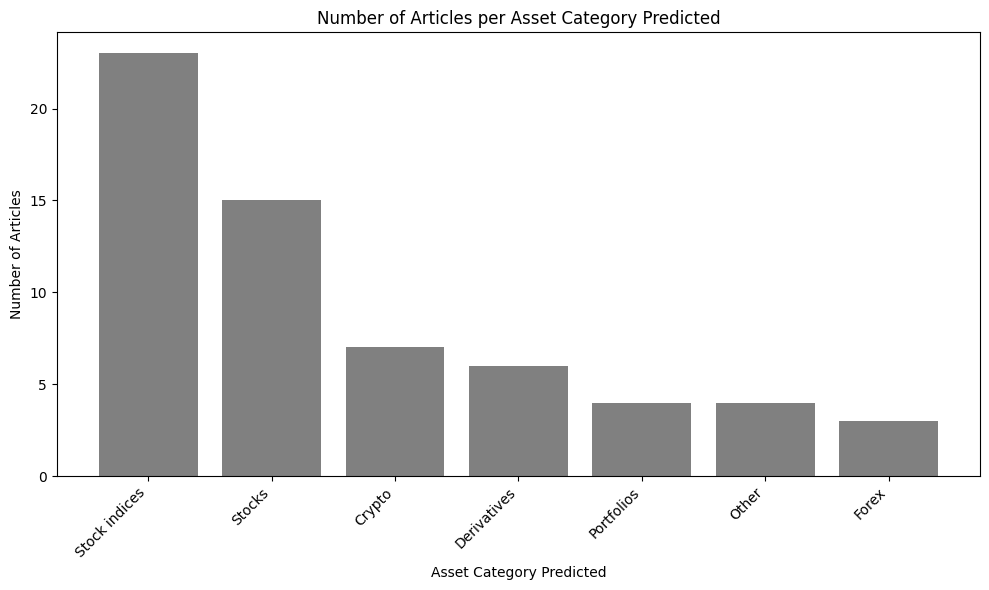
\includegraphics[width=1\linewidth]{Images/articles_per_asset_type_predicted.png}
    \caption{Asset type predicted}
    \label{fig:asset_type_predicted}
\end{figure}
\makeatletter

%%%
%% Hva skal skrives om her?
%%
%% Kanskje:
%% - Hvilket problem prøver man å løse ved å predikere asseten?
%% - Hvorfor er usikkerhetsestimater nyttige i denne konteksten?
%% - Hva har blitt gjort i artiklene i samplet?
%%
%% Bare se an hvor interessant det blir når vi har prøvd litt og så evt. flytte til descriptive statistics hvis det ikke er så interessant.
%%%



% --------- Stocks -------------------------------%
\subsubsection{Stocks}
Individual stocks are the most frequently analyzed asset class in the sample, with 21 articles. While a few studies focus on a single stock, the majority apply a common model to multiple stocks. Accurately predicting stock prices has proven challenging due to market efficiency \parencite{fama1970efficient}, which posits that prices fully incorporate all available information. In contrast, volatility has demonstrated greater predictability \parencite{poon2003forecasting}, emphasizing the relevance of uncertainty estimation for stocks. 

Most authors are motivated by the need for accurate forecasts of individual stock fluctuations to inform investor decisions and develop trading strategies. Trading strategies rely on informed beliefs about future price movements \parencite{vuletic2024finGAN}, and accurate range predictions are valuable for risk management \parencite{Li2024DeepAR}, as improved uncertainty estimates can help investors make more informed decisions regarding individual stocks and optimize profits. As \textcite{govindasamy2014prediction} note, the main problem faced by investors is that they do not have a clear idea on what stocks to invest in to maximize profits.  

Some studies do however study how external factors impact the uncertainty of individual stocks across countries and sectors differently \parencite{chandra2021bayesian, soleymani2022longterm}. Notably, \textcite{chandra2021bayesian} select stocks from mutiple counties to analyze the COVID-19 pandemic effect on different individual stock's fluctuations, highlighting the varying impact global events on asset-level uncertainty and underscoring the need for robust uncertainty quantification. 

% --------- stock Indicies-------------------------%
\subsubsection{Stock indices}
Stock indices are the second most prevalent category in the sample with 20 articles, with American, European and Asian indices dominating. Since indices are typically composed by multiple stocks from different sectors, they are generally less volatile than individual stocks and more indicative of the general state of the economy \parencite{sezer2020financial}. Therefore, uncertainty quantification can provide valuable insight into underlying market volatility. 

While most authors are motivated by the trading purposes of accurately forecasting indices, given that they are among the most important assets in the financial market, any of those emphasizing uncertainty are motivated by underlying market investigation. \textcite{Suphawan2022gpr} point out that stock price indices reflect the market, and reliable uncertainty estimates are therefore valuable in financial decision-making and risk management \parencite{Wang2021gpr}. Furthermore, \textcite{Wang2021gprensemble} state that accurate forecasts of fluctuation characteristics of indices can help government departments to timely and effectively supervise and guide the market to avoid financial risk. In addition, with the globalization of the world economy, several studies are focused on the interdependencies between indices in different across the world \parencite{cao2019multi, Malagrino2018Forecasting}, making uncertainty estimates important to support risk management strategies on international scale.

% --------- Portfolios --------------------------%
\subsubsection{Portfolios}
9 articles in the sample focus on portfolios, referring to articles where the authors explicitly construct combinations of assets and forecasts its value, returns or assess risk measures. Across the studies, the primary motivation is to maximize portfolio returns while incorporating financial risk measures to assess and manage uncertainty. In addition, \textcite{Risk2018gpr} actualize regulatory compliance with Solvency II requirements in insurance for risk assessment at the 99.5\% confidence-level. \textcite{kim2023portfolio} highlight the motivation for using a probabilistic model as opposed to deterministic models due to distributional outputs, and as the variance of predicted distributions can signify uncertainty, the models maximizing returns and minimizing risk in parallel. Most studies derive quantile-based risk measures from distributional outputs, with \textcite{Fatouros2023DeepVaR, arian2022encoded, caprioli2023quantifying} focusing on VaR, and  \textcite{Risk2018gpr, Min2023BlackLitterman} extend use to TVaR and CVaR respectfully. 

% --------- Crypto -----------------------------%
\subsubsection{Cryptocurrencies}
There are 5 articles in the sample focused on forecasting cryptocurrencies, with Bitcoin being the most prevalent subject. Recent studies of the most frequently traded cryptocurrencies suggest that the markets are becoming increasingly efficient and interconnected, although efficiency and volatility fluctuate significantly over time \parencite{noda2021evolution, liu2019volatility, gupta2022empirical}. This evolving efficiency makes the integration of cryptocurrencies into investment portfolios more attractive to investors.

Despite increasing efficiency, most articles in the sample are motivated by the fluctuating volatility and its implications for risk management. \textcite{Golnari2024Cryptocurrency} note that rapid value fluctuations make accurate prediction challenging and emphasize that understanding the inherent uncertainty in predictions and price dynamics is crucial for effective risk management in investment and trading. Similarly, 
\textcite{Almeida2024RiskForecasting} highlight the substantial loss potential in crypto markets, underscoring the paramount importance of understanding risk and implementing effective risk management strategies. \textcite{cocco2021predictions} state that the high volatility of cryptocurrencies, has made trading highly relevant in recent years, suggesting speculation may be profitable. 


% --------- Forex -----------------------------%
\subsubsection{Forex}
% Liquid market driven by many macroecomonic factors. Prob.AI applied to capture exchange rate flutions and uncertainty from complex international dynamic... essetion for both long and short term currency risk mangement
% Use forex volatility as external input to stock forecasting .. 
Foreign exchange (Forex) is one of the most liquid and interconnected assets globally. The market is driven by several macroeconomic factors, geopolitical dynamics and international trading making uncertainty quantification challenging \parencite{Rossi2013ExchangeRP}.
In the sample, six articles address forex forecasting. They usually predict forex as part of several different application scenarios for testing their model, often motivated by inter-market dependencies, rater than uncertainty in the forex market alone. 
\textcite{li2010stochastic} argue that vagueness and uncertainty often present in certain data cannot effectively be managed by traditional models and necessitates probabilistic models to handled the forecasting challenges and integrate uncertainty in predictions \parencite{Moller2007Uncertainty, li2010stochastic}. 
\textcite{cao2019multi} highlight that understanding cross-market influences, like those between forex is essential for international risk management, where uncertainty estimates help to understand forex response to global market dynamics.  

\textcite{Papaioannou2022gpr, Platanios2014gpr, 
tang2024period} all emphasize the importance of uncertainty estimates in financial market forecasting, motivated by the complex, high-volatility nature of the markets like forex markets. Their studies are motivated by making forecasting under unpredictability better and improve risk management ability to take informed decisions in interconnected markets.  


% --------- Derivatives -----------------------%
\subsubsection{Derivatives}
Nine articles in the sample focus on derivatives, which in this context are financial instruments whose value are derived from the underlying asset, such as stocks, bonds or indices. 

The most frequent derivative among the articles are volatility indices. \textcite{hortua2024forecasting, Daniali2021} analyze the VIX, while \textcite{Tian2023} extend their analysis to include the COEVI and TYVIX. Volatility indices, and the VIX in particular, are recognized as good indicators of investor sentiment and market turbulence, making it valuable for asset managers and regulators to foresee, but it remains difficult to forecast \parencite{hortua2024forecasting}. Probabilistic forecasts  of these indices could therefore be valuable to quantify the uncertainty around future volatility.

Options are another commonly derivative, with studies such as \textcite{Park2014gpr} focusing on KOSPI options, \textcite{DeSpiegeleer2018gpr} S\&P options and \textcite{tang2024period} different ETF options. \textcite{Park2014gpr} highlight a key limitation of traditional models like Black-Scholes: their inability to provide predictive distributions of the option prices. Probabilistic models, such as the GPR employed in their study, address this gap by offering predictions with uncertainty improving risk assessment - a primary motivation for the authors. 

Lastly, the sample include studies on credit default swap spreads \parencite{Law2017Practical} and capped volatility swaps \parencite{Hocht2024gpr}. 


\subsubsection{Commodities}
There are four articles in the sample that predict commodities, either gold or oil prices, or commodity futures based on the exclusion criteria outlined in Section \ref{sec:methodology}. 

\textcite{Wang2024GoldForecasting} is motivated by developing a probabilistic forecasting framework for gold prices to golds market dynamics. The authors point out golds important position in the global economy, both as a physical commodity and as a financial asset that has significant macroeconomic influence \parencite{Wang2024GoldForecasting, Pierdzioch2014Efficiency, Pierdzioch2014International}, and that gold cannot be effectivity foretasted using point estimates with reliable and credible forecasts, in particular in situation with extreme uncertainty \parencite{Wang2024GoldForecasting, Li2012Quantile}. Similar motivation can be seen in \textcite{Law2017Practical} where they predict futures of gold and crude oil.  

\textcite{li2020multivariate} predict agriculture future price, highlighting the importance of accurate forecast in order to reduce market uncertainty and support decision making in agriculture risk management and crop insurance programs, and being vital for policymakers and investors \parencite{li2020multivariate, Wang2017Performance, Ouyang2019Agricultural}. They also note that traditional models often assume independent variables and normal distribution but underscores that this assumption do not align with the real market conditions for commodities. 


\subsubsection{Bonds}
\textcite{Law2017Practical} utilize a Bayesian framework for a Support Vector Regression (SVR) to predict various financial assets, including bond yields. The authors predict both US 10-year treasuries and UK Gilt 10-year bond yields. They do not discuss motivation for using a probabilistic framework for predicting the bond yields specifically. 



% --------- Conclusion -----------------------%


% Write that we dont assess bonds.  

\subsubsection{Conclusion} % deside if we need this
Table \ref{table:conclusions_by_asset_classes} provides a summary of the primary focus and motivations of the authors making uncertainty estimates for the studied asset classes.

\begin{table}[H]
    \centering
    \caption[Summarizing conclusions by asset classes]{Summarizing conclusions by asset classes}
    \label{table:conclusions_by_asset_classes}
    \small
    \begin{adjustbox}{width=0.5\textwidth,center}
    \begin{tabular}{p{0.1\textwidth}p{0.40\textwidth}}
        \toprule
        \textbf{Asset Class} & \textbf{Conclusion} \\
        \midrule
        Stocks & \smallbullet{Enhance distributional stock forecasts for better trading and risk management} \smallbullet{Quantify how external factors impact stock uncertainty across markets} \\
        \addlinespace
        \hdashline[0.2pt/3pt]
        \addlinespace
        Stock indices & \smallbullet{Index uncertainty can reflects broader market volatility, aiding in financial decision-making} \smallbullet{Understanding interdependencies between international indices to enhance cross-border risk management} \\
        \addlinespace
        \hdashline[0.2pt/3pt]
        \addlinespace
        Portfolios & \smallbullet{Maximizing portfolio returns while leveraging uncertainty estimates for risk management} \smallbullet{Probabilistic models offer distributional outputs that support risk measures like VaR} \\
        \addlinespace
        \hdashline[0.2pt/3pt]
        \addlinespace
        Crypto & \smallbullet{High volatility of cryptocurrencies emphasize uncertainty quantification for risk-aware trading and investment} \smallbullet{Understanding fluctuating market dynamics for managing potential losses and leverage speculative opportunities} \\
        \addlinespace
        \hdashline[0.2pt/3pt]
        \addlinespace
        Forex & \smallbullet{Highly liquid and interconnected asset global driven by multiple factors making uncertainty quantification important for short- and long-term risk and trade management} \smallbullet{Cross-market dependencies necessitate probabilistic models for enhanced uncertainty estimation} \\
        \addlinespace
        \hdashline[0.2pt/3pt]
        \addlinespace
        Derivatives & \smallbullet{Probabilistic models address limitations of traditional methods  providing predictive distributions} \smallbullet{Volatility indices and option studies most prevalent} \\
        \addlinespace
        \hdashline[0.2pt/3pt]
        \addlinespace
        Commodities & \smallbullet{Uncertainty estimation important for strategic decisions making in i.e energy investment and agriculture risk management and policymakers} \smallbullet{Probabilistic models improve forecasting accuracy for commodities with non-stationary and non-linear characteristics} \\
        \addlinespace
        \addlinespace
        \bottomrule
    \end{tabular}
    \end{adjustbox}
\end{table}



%----------------------------------------------------%
% --------- Analysis by Type of Uncertainty-----------%
%----------------------------------------------------%

%Remember to include somehow the measures/how autors assess their uncertainty estimate - we also need to evaulate the strenght of these estimates, but that might be conclusion %


\subsection{Analysis by Type of Uncertainty}
\label{sec:analysis_by_type_of_uncertainty}

All the proposed models in our sample can provide estimates with some form of quantified uncertainty. However, the type of uncertainty and how the authors interpret it vary significantly. As shown in Figure \ref{fig:uncertainty_quantification_by_type_and_assessment}, many authors neither use nor interpret the uncertainty estimates at all. When they do present uncertainty estimates, they usually treat them as total uncertainty, without assessing whether it arises from modeling limitations (epistemic uncertainty) or from the inherent volatility of the underlying asset (aleatoric uncertainty). This distinction is crucial for investment decisions because it's important to know whether the uncertainty is due to an unreliable model or a risky asset.

Furthermore, only a minority of articles evaluate the quality and usefulness of the uncertainty estimates, and even fewer compare these estimates against traditional models. The following sections explore the various ways uncertainty quantification has been used in the sample articles, the financial relevance of each type of uncertainty, and how different uncertainty estimates have been and can be assessed. Summarizing results and conclusions by type of uncertainty are shown in Table \ref{table:conclusions_by_uncertainty}.


\begin{figure}[H]
    \centering
    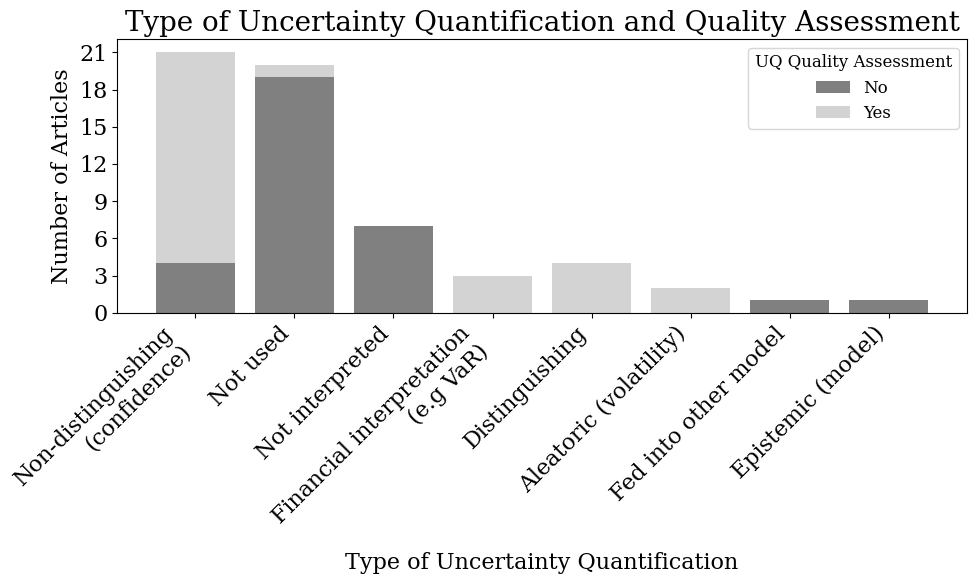
\includegraphics[width=1\linewidth]{Images/uncertainty_quantification_by_type_and_assessment.png}
    \caption{Authors' interpretation of the uncertainty estimates from the models and whether they have assessed the correctness of the uncertainty estimates}
    \label{fig:uncertainty_quantification_by_type_and_assessment}
\end{figure}


%--------------------Not Interpreted or not used-------------------------%
\subsubsection{Not used}

Among the 61 articles in the sample, 19 do not in any way mention or illustrate that their models can produce outputs with uncertainty, even though they are utilizing models that inherently have the capability. In most of these cases, the authors' motivations for using probabilistic models are not clear, but some authors show that a probabilistic model can produce better point estimates \parencite{Daniali2021, Papaioannou2022gpr, Park2014gpr}, while others apply probabilistic principles to improve generalization \textcite{jang2018generative}.

\subsubsection{Not interpreted}

In 7 articles, the probabilistic outputs from the model are presented, but not interpreted or assigned any financial or technical meaning. Generally, this is simply due to a non-existing focus on uncertainty estimation, but rather accuracy of point predictions \parencite{DeSpiegeleer2018gpr} or accuracy of category classifications e.g. \parencite{Malagrino2018Forecasting, Zhang2016}


%-----------------------Epistemic-----------------------------%
\subsubsection{Epistemic (model-uncertainty)}
Epistemic uncertainty arises from uncertainty about which model or set of weights is correct.

Only one article in the sample \parencite{Hassan2024Bitcoin} interprets the quantified uncertainty as purely epistemic. Hassan proposes a Bayesian LSTM model tasked with predicting the price of Bitcoin. Specifically, Monte Carlo dropout is used to estimate the LSTM weights—a Bayesian inference technique introduced by \textcite{gal_ghahramani_2015}. This technique involves keeping dropout active during prediction time, allowing the model to generate as many predictions as desired. These predictions form a distribution that captures the model's uncertainty about which weights are optimal. By default, this approach estimates only epistemic uncertainty, without capturing latent volatility or providing a total uncertainty estimate, unless specifically designed to do so.

As with other uncertainty estimates, it is possible to test the adequacy of epistemic uncertainty estimates by constructing confidence intervals and examining the coverage, but such as test was not conducted in this article.


%-------------------Aleatoric-------------------------------%
\subsubsection{Aleatoric (volatility)}
There are only four articles in the sample that interprets the quantified uncertainty as exclusively aleatoric uncertainty, meaning the underlying data uncertainty, which in finance is referred to as the latent volatility. This is of major interest within finance, as it is the primary measure for risk, and often the basis for deriving other risk measures \parencite{Brooks2003VolatilityFF}.

Two of the articles in the sample \parencite{arian2022encoded, xing2019sentiment} do this through the use of Variational Auto-Encoders, that can generate non-parametric output distributions through repeated sampling, thereby capturing a spectrum of potential future scenarios, as described in \ref{sec:distribution}.

The two other articles use Quantile Regression Deep Learning \parencite{Wang2024GoldForecasting} that quantifies aleatoric uncertainty through estimating several quantiles of the underlying distribution, and MaxEnt-modeling which is an application of the maximum entropy principle \parencite{Horenko2020}.

Testing the quality of aleatoric uncertainty estimates can be conducted similar to testing the quality of financial risk measures in \ref{sec:financial_risk_measures}. It should be ensured that the model on average produces uncertainty estimates of the correct magnitude (i.e. coverage testing) and that it is able to capture the heteroscedasticity of financial time series (i.e. conditional coverage testing). Additionally, it is useful to assess performance relative to traditional models using scoring metrics such as coverage relative to width, negative log-likelihood (NLL), and interval scores.

All four mentioned articles apply relevant scoring metrics and all except \textcite{Wang2024GoldForecasting} compare their results to GARCH and similar models. However, only \parencite{arian2022encoded} and \parencite{Horenko2020} conduct statistical tests for adequacy.

Some of the models that will be discussed in Section \ref{sec:total_uncertainty} below also use techniques that can capture aleatoric uncertainty, but they do not quantify it separately from the epistemic uncertainty.

%-----------------------Total uncertainty--------------------------%

\subsubsection{Total uncertainty (non-distinguishing)}
\label{sec:total_uncertainty}

Out of the 35 articles where the authors interpret uncertainty, the majority (18) treat it as total uncertainty. In this context, the uncertainty is supposed to indicate how likely it is that the prediction is accurate. However, they do not identify the sources of uncertainty—epistemic and aleatoric—and it remains unclear how much uncertainty comes from each source. The authors often state that knowing the model's confidence in its predictions is useful in investment decisions. However, not distinguishing between aleatoric and epistemic uncertainty limits the models' usefulness in investment decisions because investors cannot determine whether the uncertainty in the predictions stems from the inherent riskiness of the underlying assets or from a poor model fit.

Additionally, many authors use uncertainty quantification techniques that are unsuitable for determining total uncertainty. For example, six articles in this category employ probabilistic AI models based on Bayesian methods. This approach is debatable because, in Bayesian models, uncertainty is inherently tied to the model's specification rather than the data itself. For instance, Bayesian neural networks treat the network weights as random variables, so any prediction uncertainty arises directly from the uncertainty in these weights. As a result, these models are inadequate for capturing uncertainty in financial time series, where latent volatility evolves over time. To address this limitation, models must be explicitly designed to account for such dynamics—for instance, by constructing a Bayesian neural network that predicts both an expected price and variance. None of the six mentioned articles take such an approach.

One possible explanation for this modeling flaw is that most articles in the sample are authored by researchers from computer science rather than finance disciplines (see Figure \ref{fig:author_faculty_origin}). As a result, they may overlook the importance of heteroscedastic noise in finance. Another explanation is that, despite the use of probabilistic AI, many studies focus primarily on the accuracy of their point predictions, treating uncertainty estimates as extra benefits of their modeling approach. This hypothesis is supported by the minimal discussion of uncertainty estimates in many articles.

Among the articles in this category where the uncertainty estimates have been evaluated, assessment typically involves coverage probabilities or portfolio performance based on these estimates (see Table \ref{table:evaluation_criteria}). While both metrics are informative, they are insufficient to conclude on the practical utility of these uncertainty measures in finance. Coverage probability alone overlooks heteroscedasticity \parencite{Christoffersen1998}, while portfolio performance is sensitive to random events when evaluated over a limited time period \parencite{barras2010}.

Models quantifying total uncertainty can be compared using metrics like coverage and uncertainty magnitude. However, the absence of comparable traditional econometric models complicates the evaluation of their contributions to the field. Among the 18 articles in this category, only \textcite{Platanios2014gpr} compares their total uncertainty estimates to GARCH. Although they report superior RMSE against squared returns, this comparison may be inappropriate, as GARCH only estimates aleatoric uncertainty, and minimizing RMSE against squared returns is not the primary objective of GARCH \parencite{BOLLERSLEV1986GARCH}. The remaining 17 articles benchmark uncertainty estimates solely against other AI/ML models developed by the authors or do not conduct benchmarking at all. This makes it difficult to assess whether the proposed models provide valuable contributions to the field in terms of effective uncertainty quantification.

\subsubsection{Both epistemic and aleatoric uncertainty}

Only five articles estimate both epistemic and aleatoric uncertainty and distinguishes between the two. This is beneficial in a financial context as the user gets information both on the model's confidence and on the underlying riskiness of the asset. Additionally, it is beneficial in a model training context, as the researchers can focus on minimizing the epistemic uncertainty, while making the aleatoric uncertainty as accurate as possible.

\textcite{Risk2018gpr} uses a GPR, which naturally quantifies epistemic uncertainty, but modifies the regression equation to introduce a conditional variance term, similar to in GARCH, thus also capturing aleatoric uncertainty. This way, they can capture both sources of uncertainty while quantifying them separately. Unfortunately, they do not perform statistical adequacy tests, nor do they benchmark against GARCH, making it difficult to judge whether this approach is promising.

In \textcite{hortua2024forecasting}, they use a BNN that outputs both an expected price and an aleatoric variance estimate for the VIX. Since the BNN naturally quantifies epistemic uncertainty, they are able to capture both types of uncertainty. They also apply calibration techniques to make the uncertainty estimates more accurate and show through the use of calibration diagrams that the calibrated predicted quantiles are closer to the true proportion of values below each quantile than the uncalibrated ones. The best performing model achieves a scaling factor 0.9859, close to the optimal value of 1, but they do not assess whether the scaling factor is time-independent or if it breaks in high-volatility periods.


\textcite{Park2024UncertaintyAware} present RSMAN, a model that quantifies both aleatoric (market) and epistemic (model) uncertainty separately. Aleatoric uncertainty, reflecting market risk, is estimated through quantile regression, while epistemic uncertainty, indicating model confidence, is gauged by detecting outliers in unusual market conditions. These separate estimates allow researchers to reduce epistemic uncertainty, for instance by gathering more data, while ensuring that aleatoric estimates accurately reflect inherent market volatility. They show the usefulness of this approach by employing a portfolio construction strategy that takes both types of uncertainty into account, but in different ways, outperforming other benchmarked portfolio strategies. However, they do not conduct any other tests.

\textcite{tegner2021probabilistic} employ Gaussian Process Regression (GPR) to predict the implied volatility surface, which serves as an estimate of aleatoric uncertainty. Given the nature of GPR, the model also quantifies epistemic uncertainty in its predictions. However, the accuracy evaluation primarily compares predicted values to actual future implied volatilities, rather than directly assessing the uncertainty estimates.

In \textcite{Parker2021BayesianHeteroskedastic} the target variable is the log of squared returns, a proxy for true volatility, and their Bayesian model structure allows them to capture epistemic uncertainty. The model achieves a perfect coverage probability of 50\% on a 50\% confidence interval, while GARCH achieves a seemingly uncalibrated 100\%, raising questions about the quality of the test.

In conclusion, several interesting approaches are taken to separate epistemic and aleatoric uncertainty, but the evaluation of the uncertainty estimates is limited. 

\subsubsection{Fed into other model}

In \textcite{soleymani2022longterm} use the probabilistic output from a BNN to model the underlying distribution of data, predicting drift and volatility parameters for each point used as input in a Feynman-Dirac integral. The authors do not assess these parameters, and do not try to model them using benchmark methods. 

\begin{table}[H]
    \centering
    \caption[Evaluation Criteria for Uncertainty Quantification]{Assessment Criteria for Uncertainty Estimates}
    \label{table:evaluation_criteria}
    \small
    \begin{adjustbox}{width=0.5\textwidth,center}
    \begin{tabular}{p{0.1\textwidth}p{0.12\textwidth}p{0.22\textwidth}p{0.06\textwidth}}
        \toprule
        \textbf{Evaluation Criteria} & \textbf{Description} & \textbf{Measures} & \textbf{Articles\tablefootnote{See Appendix \ref{appendix:descriptive_table_of_all_articles} for full overview of all articles }} \\
        \midrule
        Coverage Probability & Measures how often values fall within a given predictive interval & Coverage probability, Prediction interval coverage probability (PICP), Mean Coverage (MC) & 11 \\
        \addlinespace
        \hdashline[0.2pt/3pt]
        \addlinespace
        Width-Coverage scores & Combines trade-off between interval width and coverage  & Continuous Ranked Probability Score (CRPS), Average Interval Score (AIS), Winkler Score, Coverage Widthbased Criterion (CWC), Mean width divided by coverage probability & 7 \\
        \addlinespace
        \hdashline[0.2pt/3pt]
        \addlinespace
        Interval Width metrics & Measures the width of predicted intervals & Forecasting Interval Normalized Average Width (FINAW), Prediction Interval Normalized Average Width (PINAW), Semi-interval metric, MWP (Mean width percentage) & 6 \\
        \addlinespace
        \hdashline[0.2pt/3pt]
        \addlinespace
        Calibration metrics & Evaluate how well predicted probabilities or uncertainty estimates align with observed outcomes & Dynamic Quantile (DQ), Quantile loss (QL), Expected Calibration Distance (ECD), Expected Calibration Error (ECE), Root Mean Squared Calibration Error (RMSCE) & 6 \\
        \addlinespace
        \hdashline[0.2pt/3pt]
        \addlinespace
        Correlation \&error metrics & Measures the relationship between predicted uncertainty and actual errors & Correlation between uncertainty and prediction error, Success rate, Negative log-likelihood (NLL), Area Under the ROC Curve (AUROC), RMSE (against squared returns) & 6 \\
        \addlinespace
        \hdashline[0.2pt/3pt]
        \addlinespace
        Entropy \& Variance metrics & Analyzes the distribution or intervals entropy and variance & Entropy of probability distribution, Kriging variance, Mean Squared Error of Variance (MSEV), Simulation variance & 5 \\
        \addlinespace
        \hdashline[0.2pt/3pt]
        \addlinespace
        Portfolio \& performance metrics & Evaluates the impact of predictive uncertainty on portfolio construction and performance & SVaR, Sharpe ratio, Portfolio construction and evaluation & 5 \\
        \addlinespace
        \hdashline[0.2pt/3pt]
        \addlinespace
        Christoffersen's test & Evaluates the conditional coverage of predictive intervals & Unconditional Coverage test, Independence test, Conditional Coverage test & 3 \\
        \addlinespace
        \hdashline[0.2pt/3pt]
        \addlinespace
        Kupiec's test &  Evaluates the unconditional coverage of predictive intervals & Kupiec's test & 3 \\
        \addlinespace
        \hdashline[0.2pt/3pt]
        \addlinespace
        Other Tests & Test that do not fit in the aforementioned categories & Largest eigenvalue in correlation matrix test  & 2\\
        \addlinespace
        \bottomrule
    \end{tabular}
    \end{adjustbox}
\end{table}




%----------------------Conclusion----------------------------%
\subsubsection{Conclusion} % deside if we need this
Table \ref{table:conclusions_by_uncertainty} summarize the the key findings from the analysis by type of uncertainty.
\begin{table}[H]
    \centering
    \caption[Summarizing conclusions by type of uncertainty]{Summarizing conclusions by type of uncertainty}
    \label{table:conclusions_by_uncertainty}
    \small
    \begin{adjustbox}{width=0.5\textwidth,center}
    \begin{tabular}{p{0.1\textwidth}p{0.40\textwidth}}
        \toprule
        \textbf{Type of Uncertainty} & \textbf{Conclusion} \\
        \midrule
        Not used & \smallbullet{Many models capable of uncertainty estimates are used merely for point predictions, even though they have the capability} \smallbullet{Probabilistic models frameworks are used for enhanced accuracy, generalization, pre-processing or optimization }  \\
        \addlinespace
        \hdashline[0.2pt/3pt]
        \addlinespace
        Not interpreted & \smallbullet{Some present probabilistic outputs from the model, but do not interpret or assign any financial or technical meaning to the uncertainty. Instead the focus remains on prediction accuracy and not on uncertainty estimation} \\
        \addlinespace
        \hdashline[0.2pt/3pt]
        \addlinespace
        Epistemic (model-uncertainty) & \smallbullet{Only one paper presents a model that only quantifies epistemic uncertainty, but no test for adequacy of the uncertainty estimate was conducted}  \\
        \addlinespace
        \hdashline[0.2pt/3pt]
        \addlinespace
        Aleatoric (volatility) & \smallbullet{Four papers interpret the quantified uncertainty as exclusively aleatoric } \smallbullet{Performance of these models are evaluated with scoring metrics and conditional coverage but adequacy tests are failed or not used}  \\
        \addlinespace
        \hdashline[0.2pt/3pt]
        \addlinespace
        Total uncertainty (non-distinguishing) & \smallbullet{Most authors do not distinguish between types of uncertainty in their estimates, but instead estimate total uncertainty} \smallbullet{Lack of distinction limit insight into whether the uncertainty is due to inherent asset risk or model reliability}  \\
        \addlinespace
        \hdashline[0.2pt/3pt]
        \addlinespace
        Both epistemic and aleatoric uncertainty & \smallbullet{Four articles quantify both epistemic and aleatoric uncertainty, providing understanding of both model reliability and inherent asset risk} \smallbullet{Interesting approaches are taken to distinguish, but the evaluation of the uncertainty estimates is limited}  \\
        \addlinespace
        \hdashline[0.2pt/3pt]
        \addlinespace
        Fed into other model & \smallbullet{Two papers use probabilistic outputs as input or labels for further modeling, like for predicting financial parameters or clustering risk status} \smallbullet{The secondary uses uncertainty are not interpreted or benchmarked, limiting insights}  \\
        \addlinespace
        \addlinespace
        \bottomrule
    \end{tabular}
    \end{adjustbox}
\end{table}

% ---------------------------------------------------------------%
% --------------------------Discussion --------------------------%
% ---------------------------------------------------------------%


\subsection{Discussion}
\label{sec:discussion}
This section will analyze the results in relation to each of the research questions presented in Section \ref{sec:introduction}.
% go through each reserach question and answer explicitly



\textbf{Summarize to what extent and in what way existing research are using uncertainty estimates from probabilistic AI models as measures of volatility or model uncertainty, or as financial risk measures for financial time series}\nopagebreak

Throughout this review we have seen that while the field of probabilistic AI for financial time series remains relatively small and fragmented, it is in rapid development. Commonly employed models discussed in section \ref{sec:analysis_by_model} include Bayesian Neural Networks (BNNs), Gaussian Regression Processes (GPRs) and probabilistic Recurrent Neural Network (RNN) extension. The primary focus of existing research seems to concern improving point prediction accuracy for different assets, and the potential for uncertainty estimation is underutilized. Out of the 61 articles reviewed, only 26 make a meaningful interpretation of uncertainty estimates generated by their models, and 23 of these somehow assess the quality of their estimates, while 35 studies do not use or interpret uncertainty estimates at all. 

Section \ref{sec:analysis_by_type_of_uncertainty} reveal that the majority of studies (18) interpret uncertainty estimates created as total uncertainty in predictions, rather than as a measure of volatility (aleatoric) or distinguishing between uncertainty types. Only 8 articles explicitly interpret uncertainty estimates as volatility, four of which distinguish between aleatoric and epistemic uncertainty and four only estimate aleatoric. No specific models or approaches seem to dominate among these. Use of uncertainty estimates from probabilistic AI models as a measure of volatility is thus limited. 

The analysis above further show that there is inadequate benchmarking and testing of the uncertainty estimates generated. Most authors use accuracy tests to show the superiority of their model in point predictions (although few compare to traditional models), but most fail to test their uncertainty estimates at all. Of those that do, the estimtes are usually not compared to an econometric model, nor does a standardized common testing procedure exist across the articles.  
Standardized benchmarks or frameworks could help quantify true value of the estimates in a financial context.

\textbf{Analyze researchers' motivation for making predictions with uncertainty and how it differs for different asset classes}\nopagebreak

A primary motivation for authors using probabilistic models across asset classes is to estimate uncertainty without having to assume any underlying distribution of data when employing non-parametric models. Traditional models usually rely on normality assumptions, a suboptimal restriction given the documented deviations of financial data from normal distribution. Additionally, several researchers highlight the self-learning and noise-tolerant capabilities of probabilistic and machine learning models.

The motivations for making predictions with uncertainty estimates also vary among the asset classes, and are primarily influenced by the unique market characteristics and investor needs inherent in each class. For assets known to have high volatility, like individual stocks or cryptocurrencies, the authors seem motivated mainly by the need to manage risk for investors and enhancing trading strategies. The frequent price fluctuations of these assets underscore the importance of accurate uncertainty estimation, both to inform investment decisions and mitigate potential losses or facilitate speculation, a main motivational factors of the authors. 

Risk management considerations for investment and trading is also the primary motivation for researchers assessing stock indices. However, given that indices like the S\&P 500 closely represent overall market performance and conditions, some researches extend their motivations for uncertainty estimates of stock indices to encompass an enhanced understanding of underlying market volatility and systematic risk. Additionally, in Forex and large international indices, some researches are motivated by understanding global interconnections and cross-market influences through uncertainty estimations.

For the researchers assessing portfolios, the primary motivation lies in  the need for uncertainty estimations for financial risk measures and regulatory compliance. Most studies construct measures like VaR, utilizing distributional output from the probabilistic models in an attempt to provide more accurate risk assessment of portfolios.

\textbf{Compare how promising probabilistic models' capabilities are compared to other machine learning models and traditional econometric models in uncertainty estimation}\nopagebreak

There are only 8 models in the sample where created uncertainty estimates are benchmarked against traditional models. In 7 of these articles authors benchmark against GARCH variants, and in 4 cases does the proposed model clearly outperform the traditional one. These models are the DeepVaR proposed by \textcite{Fatouros2023DeepVaR}, the GPMCH by \textcite{Platanios2014gpr}, the ESVM by \textcite{Parker2021BayesianHeteroskedastic} and the SAVING model by \textcite{xing2019sentiment}. However, there are 10 articles in which the authors compare the uncertainty estimate of their model with another machine learning model, where only 2 also compare against a traditional econometric model. All models outperform the machine learning model baselines. These findings suggest lacking and unsatisfactory benchmarking against traditional econometric like GARCH, making it difficult to draw definitive conclusions.

When it comes to point predictions there are 25 articles where the researchers benchmark their points predictions against traditional models. Of these, 23 show clear superior performance, demonstrating promise in accurate predictive power. A total of 44 articles benchmark their model against other machine learning models, and 36 of them outperform their benchmarks. Once again, this suggest a bias towards comparing with other machine learning models rather then traditional econometric models. Even though these results demonstrate promising accuracy for point predictions for probabilistic models, there is strong evidence of publishing bias in finance, making it difficult to conclude on the soundness of these results \parencite{Kim2015SignificanceTI}.

Importantly, researchers typically only compare models on accuracy metrics, which is not necessarily sufficient for determining which model is the most useful in practice. For financial stakeholders, understanding the reasoning of the model might be as important as accuracy \parencite{Freeborough2022}. In this regard, explainable AI (XAI) is a more promising field than probabilistic AI, but there is no reason why the two cannot be combined.

In conclusion, probabilistic models seem to provide improved point predictions and have interesting properties for financial modeling, such as being able to estimate non-parametric distributions and capturing non-linear patterns. There are some models demonstrating promising results in uncertainty estimation, but limited benchmarking especially with traditional models makes it difficult to conclude on the real promise of the models.


\textbf{Investigate probabilistic models' ability to provide improved understanding of risk and volatility compared to econometric models}\nopagebreak

For investors, understanding where the source of uncertainty stems from is important for informed decision-making. The inherent ability of probabilistic AI models to distinguish between epistemic and aleatoric uncertainty offer a potential advantage in providing a better understanding of uncertainty over traditional econometric models like GARCH, which are unable to quantify epistemic uncertainty. Although only four articles explicitly leverage this capability, it highlights the promise of probabilistic models for better insights in uncertainty estimates.

Another key advantage of certain probabilistic models, highlighted by several studies, is their their ability to estimate non-parametric distributions. An inherent limitation of traditional econometric models are relying on parametric assumptions (usually normal) about the data distribution, even though most financial time series exhibit non-normality and fatter tails particularly. The flexibility of the non-parametric probabilistic models address this limitation by not having to make assumptions about the underlying distribution. Additionally, machine learning models can capture non-linear patterns in data, another advantage over econometric approaches.

Several proposed models demonstrate how probabilistic AI can simultaneously model multiple assets while accounting for their correlations, providing return predictions and uncertainty quantification for each asset or the entire portfolio. This capability is particularly valuable for understanding portfolio risk and is challenging to achieve with traditional models.

\textbf{Identify the metrics used for assessing probabilistic AI models and assess what the most appropriate metrics for assessing the quality of the produced uncertainty estimates is}\nopagebreak

Because the sample includes articles within probabilistic AI for quantifying different types of uncertainty and with different purposes, test practices vary widely.

Few papers acknowledge that their quantified uncertainty is primarily epistemic, and even fewer attempt to evaluate the accuracy of these estimates. However, epistemic uncertainty could theoretically be assessed using metrics like coverage probability.

In papers that quantify aleatoric uncertainty, through measures like volatility or VaR, evaluating the uncertainty estimates is more common. However, we find that testing procedures vary extensively, and no standardized frameworks seem to be established. Authors often apply some, but rarely all, of the following tests:

\begin{enumerate}
    \item Statistical tests for adequacy, such as Christoffersen's test, showing that the uncertainty estimates from the model can be used to construct confidence intervals with the correct coverage and where outliers are independently distributed over time
    \item Scoring functions, such as interval width, coverage relative to interval width, negative log-likelihood (NLL) etc. that can be used to compare uncertainty estimates from different models against each other
    \item Benchmarking tests against traditional models such as GARCH, using several accuracy measures
\end{enumerate}

Few authors conduct all three types of tests, despite all being necessary to judge whether a model is a valuable contribution to the field. Therefore, we propose the aforementioned list should be a standardized framework for assessing the quality of uncertainty estimates constructed using probabilistic AI models for financial time series moving forward. 

\textbf{Analyze how probabilistic AI models can be used to construct financial risk measures such as Value at Risk (VaR) and Expected Shortfall (ES)}\nopagebreak

There are 6 articles in total creating financial risk measures using probabilistic models, where tail-risk estimates for portfolios such as VaR is the most prevalent. Several authors argue that traditional parametric methods for VaR estimation are limited by explicit return distribution and linear dependency assumptions, which do not necessarily hold for financial time series \parencite{arian2022encoded,Fatouros2023DeepVaR}. Probabilistic models like Variational Auto-Encoders (VAE) and DeepAR, utilized in several articles for VaR estimation, directly address this limitation by generating probabilistic forecasts of the entire return distribution without explicit parametric assumptions. The distributional output of the models can be used directly for tail-risk estimation. Probabilistic models are thus potentially well-suited for constructing financial risk measures such as VaR or ES, and can be used to effectively address limitations of traditional models. These models due not curently consistently outperform traditional models, largely due to partially insignificant estimates, but the inherent modeling capabilities of these models--such as arbitrary distribution shapes--hold promise for future research to create better VaR estimates.

\textbf{Identify possible areas for further research}\nopagebreak

The novelty and rapid evolution of probabilistic AI for financial modeling this review highlights presents multiple key areas for future research that could be beneficial for deeper exploration in order to enhance uncertainty quantification and risk estimation in finance. 

To advance these objectives, we suggest the following summarizing recommendation for future research: 

\begin{enumerate}
    \item Probabilistic AI models capability to produce non-parametric distributions remains underutilized. Exploration of this feature with thorough testing has a lot of potential and could yield more accurate prediction in volatile conditions where parametric assumptions may not hold.
    \item Further studies should explore and test different probabilistic models to create adequate financial risk estimates such as VaR and ES, across different asset classes and market conditions.
    \item When modeling financial time series, models should always and more explicitly differentiate between epistemic and aleatoric uncertainty. This will provide clearer insights into the source of uncertainty, distinguishing the inherent asset volatility and limitations in the model.
    \item For models with the purpose of enhanced uncertainty estimates, it is critical that the aleatoric uncertainty estimates are tested with rigorous evaluation methods, e.g. with Christoffersen's test and different scoring functions, and that performance is compared across models reliably to validate the results.
    \item Research should aim to and use comprehensive and standardized testing for evaluating full predictive distributions, rather than focusing on selected quartiles (e.g. 95\% VaR) for more comprehensive model validation, similar to suggested framework proposed earlier in this section.
    \item Current probabilistic AI models are largely "black boxes" where it is difficult or impossible for users to understand the reasoning behind the predictions. Combining probabilistic AI with techniques from explainable AI could enhance the usefulness of probabilistic AI model in practice.
\end{enumerate}


%- testing different probabilistic models to create significant financial risk estimates such as VaR

%her syns jeg vi burde komme med en del tydelige recommendations for fremtidig research:

%1. man burde alltid skille mellom epistemic og aleatoric uncertainty når man modellerer finansielle tidsserier

%2. dersom man lager en modell der usikkerhet er i fokus er det kritisk at de aleatoriske usikkerhetsestimatene testes rigorously, med f.eks. en kombinasjon av christoffersen's test og scoring-funksjoner der man sammenligner med andre modeller

%3. hvis det ikke finnes allerede burde noen lage et tydelig rammeverk for hvordan man tester fulle distribusjoner, altså ikke bare f.eks. 95\% VaR men hver eneste kvantil

%4. det er veldig få artikler hvor ai-modellers evne til å produsere ikke-parametriske distribusjoner utnyttes fullt ut, det hadde vært interessant om det ble gjort i større grad og om det ble testet ordentlig

%5. Combine probabilistic AI models with traditional models like GARCH to estimate the uncertainty, where few articles propose such a hybrid model